Yeah so this next chapter we do x.y.z.


%
%\documentclass[%
% reprint,
% amsmath,amssymb,
% aps,
% prd,
%]{revtex4-2}
%
%\usepackage{graphicx}% Include figure files
%\usepackage{dcolumn}% Align table columns on decimal point
%\usepackage{bm}% bold math
%\usepackage[dvipsnames, usenames]{xcolor}
%\usepackage{acronym}
%\usepackage{hyperref}
%
%%\usepackage{hyperref}% add hypertext capabilities
%%\usepackage[mathlines]{lineno}% Enable numbering of text and display math
%%\linenumbers\relax % Commence numbering lines
%\newcommand{\sv}[1]{{\textcolor{BurntOrange}{\sf{[sv:#1]}}}\xspace}
%
%\newcommand{\chieff}{\chi_{\rm eff}}
%\newcommand{\mc}{\mathcal{M}_c}
%\newcommand{\dataset}{\{d_i\}_{i=1}^{N_{\rm obs}}}
%\newcommand{\beq}{\begin{equation}}
%\newcommand{\eeq}{\end{equation}}
%\newcommand{\nn}{\nonumber}
%\newcommand{\parint}[1]{\int {\rm d}#1}
%\newcommand{\thetaint}{\parint{\theta}}
%\newcommand{\dataint}{\int_{\mathcal{D}_{\uparrow}} {\rm d}d}
%\newcommand{\Msun}{\;M_\odot}
%\newcommand{\pp}{{\sc Power-Law + Peak}}
%\newcommand{\pr}{{\sc Power-Law Redshift}}
%
%
%\newcommand{\rednote}[1]{{\color{Red} #1}}
%\newcommand{\LIGOlabMIT}{\affiliation{LIGO, Massachusetts Institute of Technology, 77 Massachusetts Avenue, Cambridge, MA 02139, USA}}
%\newcommand{\MKI}{\affiliation{Kavli Institute for Astrophysics and Space Research and Department of Physics, Massachusetts Institute of Technology, 77 Massachusetts Avenue, Cambridge, MA 02139, USA}}
%\newcommand{\CIERA}{\affiliation{Center for Interdisciplinary Exploration and Research in Astrophysics (CIERA), Northwestern University, 1800 Sherman Ave, Evanston, IL 60201, USA}}
%
%
%\begin{document}
%%% ============================================================
%%% Thesis chapter heading (replaces journal \maketitle block)
%%% ============================================================
\chapter{Probing Correlations in the Binary Black Hole Population with Flexible Models}

\chapterauthors{Jack Heinzel$^{1}$, Sylvia Biscoveanu, Salvatore Vitale}

\begin{refsection}
\label{chapter: glitches}
%\title{...}\author{...}\maketitle  % journal header — commented out
\begin{chapterabstract}
The astrophysical formation channels of binary black hole systems predict correlations between their mass, spin, and redshift distributions, which can be probed with gravitational-wave observations. Population-level analysis of the latest LIGO-Virgo-KAGRA catalog of binary black hole mergers has identified evidence for such correlations assuming linear evolution of the mean and width of the effective spin distribution as a function of the binary mass ratio and merger redshift. However, the complex astrophysical processes at play in compact binary formation do not necessarily predict linear relationships between the distributions of these parameters.
In this work, we relax the assumption of linearity and instead search for correlations using a more flexible cubic spline model. Our results suggest a nonlinear correlation between the width of the effective spin distribution and redshift. We also show that the LIGO-Virgo-Kagra collaborations may find convincing Bayesian evidence for nonlinear correlations by the end of the fourth observing run, O4. This highlights the valuable role of flexible models in population analyses of compact-object binaries in the era of growing catalogs.
\end{chapterabstract}

\acrodef{GWTC-3}[GWTC-3]{third gravitational-wave transient catalog}
\acrodef{BBH}[BBH]{binary black hole}
\acrodef{LVK}[LVK]{LIGO-Virgo-Kagra collaboration}
\acrodef{KL}[KL]{Kullback-Leibler}
\acrodef{JS}[JS]{Jensen-Shannon}
\acrodef{GW}[GW]{gravitational wave}

% \tableofcontents

\section{Introduction}
The growing catalog of gravitational-wave observations of \acf{BBH} mergers has allowed for increasingly detailed probes of the population properties of these systems, with the ultimate goal of revealing how they form and evolve. Analysis of the \acf{GWTC-3}~\cite{LIGOScientific:2021djp} of the \acf{LVK}~\cite{TheLIGOScientific:2014jea, TheVirgo:2014hva, Aso:2013eba, Somiya:2011np, KAGRA:2020tym} found evidence for substructure in the \ac{BBH} primary mass distribution~\cite{KAGRA:2021duu, Tiwari:2020otp, Edelman:2021zkw} beyond a single power-law~\cite{Fishbach:2017zga} plus Gaussian peak~\cite{Talbot:2018cva} and for preferentially equal-mass mergers~\cite{Fishbach:2019bbm, Farah:2023swu}. The black hole spin distribution favors small~\cite{Wysocki:2018} but likely nonzero spins~\cite{Biscoveanu:2020are, Callister:2022qwb, Tong:2022iws, Mould:2022xeu, Galaudage:2021rkt, Roulet:2021hcu}, and the distribution of the spin tilts relative to the orbital angular momentum is consistent with isotropy, while the distribution of effective aligned spins indicates a slight preference towards positively aligned spins~\cite{Roulet:2021hcu, Miller:2020zox, KAGRA:2021duu, Vitale:2022dpa, Golomb:2022bon}. The merger rate evolves with redshift at a rate consistent with the cosmic star formation rate~\cite{Fishbach:2021yvy}. Taken altogether, these constraints imply that there are probably multiple formation channels~\cite{Zevin:2020gbd, Cheng:2023ddt, Wong:2020ise} shaping the \ac{BBH} population, although no definitive evidence for sub-populations with different properties has been identified~\cite{Baibhav:2022qxm, Godfrey:2023oxb, Wang:2022gnx}.

While most previous analyses of the \ac{BBH} population have relied on phenomenological population models with simple parametric functional forms, recent work has explored the use of ``non-parametric'' models like splines~\cite{Edelman:2022ydv, Golomb:2022bon}, Dirichlet processes~\cite{Rinaldi:2021bhm}, generic mixture models~\cite{Tiwari:2020otp,Tiwari:2020vym,Tiwari:2021yvr}, binned Gaussian Processes~\cite{Foreman-Mackey_2014, KAGRA:2021duu, Ray:2023upk}, and autoregressive models~\cite{Callister:2023tgi}. Despite including many more free parameters than the phenomenological models, these non-parametric models offer increased flexibility to fit the data without imposing a specific functional form. This avoids the issue of model misspecification~\cite[e.g.,][]{Romero-Shaw:2022ctb} at the cost of a clear mapping between features observed in the data and those predicted by astrophysical theory.

As the observed population of \ac{BBH} mergers grows, population analyses have moved beyond modeling the mass, spin, and redshift distributions independently towards searching for correlations between these parameters.
Such correlations are expected both within individual formation channels and due to the superposition of sub-populations forming via distinct channels~\cite{Bavera:2022mef, Bavera:2020inc, McKernan:2012rf, Stone:2016wzz, McKernan:2019beu, McKernan:2021nwk, Tagawa:2019osr, Mukherjee:2021rtw, Zevin:2022wrw, Karathanasis:2022rtr}. For example, \acp{BBH} formed via isolated binary evolution may exhibit correlations due to the relationship between metallicity and the efficiency of angular momentum transport via stellar winds. These winds remove mass and spin-down the progenitor, meaning that more massive systems would prefer higher spins. They would also be more common at high redshift, where stellar winds are less efficient because of lower metallicities~\cite{Belczynski:2017gds}.
%For example, \acp{BBH} formed via isolated binary evolution may have larger effective spins at higher redshifts due to a correlation between the orbital separation--which affects the delay time and merger redshift--and the efficiency of tidal spin-up of the black holes' stellar progenitors~\cite{Bavera:2020inc}. Such a correlation may also be imparted due to the relationship between metallicity and the efficiency of angular momentum transport via stellar winds, which remove mass and spin down the progenitor, leading to a corresponding correlation between mass and redshift~\cite{Belczynski:2017gds}. 
A mass-spin correlation is also expected for systems formed dynamically via hierarchical mergers in dense environments, since remnants of previous mergers that go on to merge again will be both more massive and rapidly spinning~\cite[e.g.,][]{PortegiesZwart:2002iks, Rodriguez:2015oxa, Gerosa:2021mno}. 

Evidence for a correlation between \ac{BBH} mass and spin was obtained using a phenomenological model where the mean and width of the distribution of effective aligned spin ($\chieff$) vary linearly as a function of the mass ratio, such that systems with more unequal mass ratios have larger effective aligned spins~\citep{Callister:2021fpo, KAGRA:2021duu}. An approach using copula density functions that ensure fixed marginal distributions in the presence of a correlation identifies this correlation at similar significance~\cite{Adamcewicz:2022hce, Adamcewicz:2023mov}. Weaker evidence using the linear correlation model also hints at a potential correlation between the effective spin distribution and the total mass and primary mass~\cite{Safarzadeh:2020mlb, Franciolini:2022iaa, Biscoveanu:2022qac}, although a broadening of the spin distribution at the highest masses can be explained due to the relative dearth of observations in this regime, leading to a more uncertain measurement~\cite{Tiwari:2021yvr}. A likely correlation between the width of the effective spin distribution and redshift has also been identified~\cite{Biscoveanu:2022qac}. Recently, using a non-parametric method, Ref.~\cite{Rinaldi:2023bbd} reports a correlation in primary mass-redshift space, arising from two sub-populations. However, some results of this work are in tension with previous population analyses, including both parametric and nonparametric methods \cite[e.g.][]{vanSon:2021zpk, Tiwari:2021yvr, Edelman:2022ydv, Callister:2023tgi}. % include if Stefan wishes.

In this work, we build upon previous methods looking for correlations between individual pairs of parameters describing the \ac{BBH} mass, spin, and redshift distributions but adopt a more flexible model for the shape of the correlation. Specifically, we assume the \ac{BBH} effective spin distribution is described by a Gaussian with an unknown mean and width, both of which may correlate with either the mass or redshift such that the shape of the correlation is given by a cubic spline. Our model recovers evidence for the previously-identified correlations between effective spin and mass ratio and redshift but prefers a nonlinear shape for the spin-redshift correlation. This result highlights the important role that flexible population models will play in identifying model misspecification as the catalog of \ac{BBH} merger observations grows. The rest of this work is structured as follows. 

In \S \ref{sec: spline probe_correlations} we briefly describe our statistical assumptions, which are standard in \acf{GW} population inference, then describe our model for probing correlations in more detail. In \S \ref{sec: spline GWTC3_results} we present the constraints on the BBH data collected thus far \cite{LIGOScientific:2021djp}, which tend to be broadly consistent with previous studies apart from some evidence for nonlinearity in the $\chieff-z$ correlation. % We also use a joint mixture-model framework to infer which parameter(s) correlate in the $\chieff$ population, which prefers the correlation to be with redshift, mass ratio, or some combination of the two. % comment out if we cut mixture model 
In \S \ref{sec: spline o4_projections} we make projections for the future: how well can nonlinearity be measured with future observations? In a pair of simulated Universes with nonlinear correlations in $\chieff-q$ and $\chieff-z$, nonlinearity does not reveal itself in the $\chieff-q$ distribution with 400 detections, but there is strong evidence for nonlinearity in the $\chieff-z$ distribution with 400 detections. While the detectability of nonlinearity ultimately is subject to how nonlinear the true correlated distribution is, we show it is possible to detect nonlinearity in the near future. 
Finally, we conclude in \S \ref{sec: spline conclusion}.

\section{Probing Correlations: Priors and Parameterization}
\label{sec: spline probe_correlations}

% \subsection{Hierarchical Inference}

% \rednote{shorten this, maybe even cut entirely}

% Broadly defined, the goal of hierarchical inference is to understand a source distribution from individual observations. There are three broad difficulties which complicates the statistical problem for GW astrophysics: choice of prior, noisy events, and selection effects. 

% The first and most mathematical problem boils down to choosing a prior. It is not clear what a general prior should be for the space of probability distributions; and beyond that, a purely uninformed prior would be infinite dimensional. The most common solution suggests parameterizing the space, choosing to model the probability distribution as superpositions of e.g. power-laws, Gaussian distributions, or whatever other distributions suit the analyst. The problem is then solved by constraining this collection of hyperparameters (denoted $\Lambda$ in this work) which describe the distribution (the power-law indices, mean and variance of the Gaussian etc.). Furthermore, when the parameterization is informed by physics, constraints on the hyperparameters correspond to constraints on underlying processes generating the sources. 

% There are other approaches which choose to solve this problem differently. For instance, one can model the probability distributions as autocorrelated processes \cite{Callister:2023tgi}, or compute the source distribution using iterative KDEs \cite{Sadiq:2021fin}. In this paper, we choose a parameterization where the hyperparameters are henceforth denoted $\Lambda$ and the distribution is written $p(\theta|\Lambda)$.
% infinite dimensional? Parameterized

% Second, individual event observations are noisy, and so the posteriors on the source parameters for an individual event have non-negligible width. This is solved by marginalizing over the uncertain parameters of each event in the likelihood \citep{Loredo_2004}. The single event terms in the hierarchical likelihood must be marginalized over the uncertainty in the event parameters. In particular, for a data observation $d$, the likelihood of that data given the hyperparameters $\Lambda$ is

% The goal of hierarchical inference is to infer an unknown distribution by combining multiple observations.
The goal of population modeling is to infer the distribution from which an ensemble of observations is drawn. This can be accomplished using hierarchical Bayesian inference, which takes a multi-stage approach by first characterizing individual observations and then combining them on a population level.
In a \ac{GW} context, these individual observations are noisy, so the statistical likelihood of observing the data given a population model $p(\theta | \Lambda)$ parameterized by $\Lambda$ must be marginalized over the possible \ac{GW} parameters \cite{Loredo_2004}
\beq
\mathcal{L}(d | \Lambda) = \thetaint \mathcal{L}(d|\theta) p(\theta | \Lambda).
\label{eq:marginalized_like}
\eeq
Here, $d$ represents the detected data, and $\theta$ represents the unknown source parameters, like the binary masses, spins, and redshift. 
% uncertain events?

Furthermore, BBHs suffer a Malmquist bias; they are not all equally detectable. To account for this bias, we must define the detection efficiency
\beq
\alpha(\Lambda) = \dataint \thetaint \mathcal{L}(d|\theta) p(\theta | \Lambda),
\label{eq:selection_eff}
\eeq
which is the fraction of events in the population $p(\theta | \Lambda)$ which probabilistically generate detectable data ($d \in \mathcal{D}_{\uparrow}$). Assuming the events are distributed in time by a Poisson process and marginalizing over the Poisson rate parameter with a uniform-in-$\log$ prior, we obtain the rate-marginalized hierarchical likelihood \citep{Loredo_2004, Farr:2013yna, Foreman-Mackey_2014, Mandel_2019, Vitale:2020aaz, Essick:2023upv}.
% selection effects?
In particular, with a collection of $N_{\rm obs}$ events with data $\dataset$ passing a detection threshold 
\beq
\mathcal{L}(\dataset | \Lambda) \propto \prod_{i=1}^{N_{\rm obs}} \frac{\mathcal{L}(d_i|\Lambda)}{\alpha(\Lambda)}.
\label{eq:hierarchical_like}
\eeq
We use this likelihood to sample from the hyperparameters $\Lambda$. In practice, we estimate the marginal integrals in Eqs. \ref{eq:marginalized_like} and \ref{eq:selection_eff} with Monte Carlo estimators, see Refs. \cite{Farr_2019, Essick:2022ojx, Talbot:2023pex} for details.

A common approach tackles % reformulates
the hierarchical inference problem by phenomenologically parameterizing the unknown source distribution as e.g. power-laws, Gaussians, etc., and inferring these hyperparameters given the data observations. Previous studies have identified simple and successful parameterization schemes; we choose the astrophysically motivated parameterizations \pp~\cite{Talbot:2018cva}
and \pr~\cite{Fishbach:2018edt} for the mass $p(m_1, q|\Lambda)$ and redshift $p(z|\Lambda)$ distributions respectively. The primary mass distribution is parameterized as a smoothed power-law plus a gaussian component, and a smoothed power-law for the mass ratio (hyperparameters are the minimum and maximum BH mass--assumed to be the same for both the primary and secondary--power-law index, low mass smoothing parameter, mean and width of the Gaussian, fraction of BBHs in the Gaussian component, and the power-law index for the mass ratio). The redshift distribution is modelled as a power-law with a single power-law index hyperparameter. 

For the spins, we project the 6 dimensional spin distribution to a one dimensional parameter $\chieff$ describing the leading order spin effect on the inspiral evolution of the binary \cite{Damour:2001,Racine:2008qv,Ajith:2009bn}, which is often the most well measured spin parameter \cite{Vitale:2016avz, Purrer:2015nkh}. 
We then model the $\chieff$ population as a truncated Gaussian distribution with a variable mean and width~\cite{Miller:2020zox, Roulet:2018jbe}
\beq 
p(\chieff|\theta, \Lambda) = \frac{1}{\sigma(\theta, \Lambda)}\frac{\phi\left(\frac{\chieff - \mu(\theta, \Lambda)}{\sigma(\theta, \Lambda)}\right)}{\Phi\left(\frac{1-\mu(\theta, \Lambda)}{\sigma(\theta, \Lambda)}\right) - \Phi\left(\frac{-1-\mu(\theta, \Lambda)}{\sigma(\theta, \Lambda)}\right)}
\label{eq:general_chieff_correlation}
\eeq
where the truncation restricts the support of the distribution to be $[-1,1]$, which reflects the physical constraint that the magnitude of $\chieff$ cannot exceed 1 for BH spins bounded by the Kerr limit. $\phi$ is the standard Gaussian and $\Phi$ is the standard error function, 
\beq
\phi(x) = \frac{e^{-x^2/2}}{\sqrt{2\pi}} \qquad \Phi(x) = \int_{-\infty}^x \phi(s)ds.
\label{eq:standard_gaus}
\eeq
This is the approach used by Refs.~\cite{KAGRA:2021duu,Safarzadeh:2020mlb,Callister:2021fpo,Biscoveanu:2022qac} to explore models where $\mu(\theta)$ and $\sigma(\theta)$ are linear functions of primary mass ($\theta = m_1$) mass ratio ($\theta = q$) and redshift ($\theta = z$) respectively. Building on this previous work, we model $\mu(\theta)$ and $\sigma(\theta)$ with spline functions.

Spline functions are becoming increasingly popular in \ac{GW} population inference, primarily because they are innately flexible and fast to evaluate, but also because they are easily parameterized by their nodes. While splines do not assume much structure, they do fail to probe structure below the scale of the node separation length. For this reason, one should include the number of nodes as a model hyperparameter or repeat the analysis varying the choice of the number of nodes. 

In this work, we use a cubic spline model, where nodes are interpolated using cubic polynomials which preserve continuity in the function and first and second derivatives at the nodes ($\mathcal{C}^2$ functions). Given node locations, this provides all but two conditions to set the four coefficients for each cubic polynomial; the final two conditions are given at the endpoints, typically imposed by setting the second derivative to zero. Defined in this way, the node positions fully determine the spline curve. Splines also have the advantage of approximate locality, meaning they can fit a structure in one region of parameter space independently of the behavior of the spline far away (separated by many nodes)~\cite{DeBoor_1976}. 

For all the inferences we present below, we use priors shown in Table \ref{tab:prior_table}. We use the {\tt Overall} samples for GWTC1 events~\cite{gwtc1_pe}, {\tt PrecessingSpinIMRHM} for the events first identified in GWTC2~\cite{gwtc2_pe} and the {\tt C01:IMRPhenomXPHM} samples for the GWTC2.1 and GWTC3 events~\cite{ligo_scientific_collaboration_and_virgo_2022_6513631, ligo_scientific_collaboration_and_virgo_2023_8177023}, and the search sensitivity estimates provided in Ref.~\cite{ligo_scientific_collaboration_and_virgo_2023_7890398}. We use the {\tt GWPopulation} package for constructing the hierarchical likelihood~\cite{Talbot:2019}, and compute Bayesian evidences while sampling the hyperposterior using the {\tt Dynesty} implementation in {\tt Bilby}~\cite{Speagle_2020,Ashton:2018jfp}. To efficiently evaluate spline functions, we use the {\tt cached\_interpolate} package introduced in Ref.~\cite{Golomb:2022bon}. In addition, because we estimate the population likelihood (Eq. \ref{eq:hierarchical_like}) with Monte Carlo integrals, there is inherent uncertainty associated with each likelihood estimate. To avoid biased inference, we cut hyperposterior samples with $\log$-likelihood uncertainty greater than 1, following the recommendation of Ref.~\cite{Talbot:2023pex}.

% \rednote{Prior table?}
\renewcommand{\arraystretch}{1.3}
\renewcommand{\tabcolsep}{0.3cm}
\begin{table*}
    \centering
    \begin{tabular}{|l||ll|}
       \hline Hyperparameter & Description & Prior \\
       \hline $\alpha$ & $m_1$ power-law index & U(-4, 12) \\
       $\beta$ & $q$ power-law index & U(-4, 7) \\
       $m_{\rm max}$ & maximum BH mass & U$(60\Msun, 100\Msun)$ \\
       $m_{\rm min}$ & minimum BH mass & U$(2\Msun, 10\Msun)$ \\
       $\delta_m$ & low-mass smoothing parameter & U$(0\Msun, 10\Msun)$ \\
       $\mu_{m}$ & $m_1$ Gaussian component mean & U$(20\Msun, 50\Msun)$ \\
       $\sigma_{m}$ & $m_1$ Gaussian component standard deviation  & U$(1\Msun, 10\Msun)$ \\
       $\lambda$ & fraction of BBHs in Gaussian component & U(0, 0.2) \\
       $\lambda_z$ & $z$ power-law index & U(-2, 10) \\
       \hline $\mu_{\chieff:n}$ & $n^{\rm th}$ spline node for the $\chieff$ mean & U$(-1,1)$ \\
       $\ln\sigma_{\chieff:n}$ & $n^{\rm th}$ spline node for the $\chieff$ standard deviation & U$(-5,0)$
       \\ \hline
       
    \end{tabular}
    \caption{Priors for each hyperparameter used in our model. The upper panel describes the standard priors, except where they are reduced to improve the sampling efficiency without cutting off the hyperposterior ($m_{\rm max}$ and $\lambda$). The lower panel describes the prior assumed for our spline parameters.}
    \label{tab:prior_table}
\end{table*}

 
\section{Correlations in \ac{GWTC-3}}
\label{sec: spline GWTC3_results}

% The population of BBHs in the Universe is likely to exhibit correlations between source parameters. Previous studies have searched for linear correlations, constraining the first order correlation. 
Using the catalog of 69 BBHs described in Ref.~\cite{KAGRA:2021duu}  passing a detection-pipeline-computed false alarm rate threshold of 1 yr${}^{-1}$, we search for evidence of nonlinear correlations between the spin distribution and the mass ratio, redshift, and the source frame primary mass (the latter is described in appendix \S~\ref{app:chieff_m}). %(because a correlation with primary mass is disfavored by the evidence, we move a discussion of primary mass correlation to the appendix). 
To do this, we model the $\chieff$ distribution with Eq. \ref{eq:general_chieff_correlation}, and present the results of the individual analyses below.

% For each parameter analyzed individually, we find varying degrees of evidence for structure in the mean or variance of the $\chieff$ Gaussian distribution, but hints of structure nonetheless. However, it is not immediately clear in which of these scenarios the correlation is bona fide or if it is spurious. Perhaps there is some confounding influence  between the correlations we studied, which generates a false positive evidence for correlation in another parameter, when analyzed with a false hypothesis. \rednote{I want to talk about a method to infer the true correlation(s), but the run doing a simultaneous fit will never finish...} % To account for this, we run a simultaneous fit for correlation between all parameters, allowing the data to inform us on which parameter should correlate. We find that in GWTC3, \rednote{there is some (?) evidence that the correlation is primarily with XXXX}

\subsection{Effective Spin Distribution and Mass Ratio}

The first correlation we explore is between $\chieff$ and mass ratio $q$, setting the mean and standard deviations to spline functions of mass ratio. We place the nodes uniformly between $q=0$ and $q=1$. Though $q\to0$ is an unphysical region of parameter space with no observations, the node at $q=0$ should be thought of as simply a parameter necessary to ensure the model is defined over the entire space, and not an \textit{a priori} statement that BBHs exist here; indeed the model $p(q\;|\;m_1, \Lambda)$ is always zero at $q=0$.
\begin{align}
\mu(\theta) &= S\left(q\;|\;(0,\mu_{\chieff:0}), ..., (1,\mu_{\chieff:N})\right) \nn \\
\ln \sigma(\theta) &= S\left(q\,|\,(0,\ln \sigma_{\chieff:0}), ..., (1,\ln \sigma_{\chieff:N})\right),
\label{eq:chieff_q_spline}
\end{align}
where $S(x\;|\;(X_1, Y_1), ..., (X_N, Y_N))$ represents the cubic spline function in the variable $x$ passing through the nodes with $x$ coordinates $X_1 < X_2 < ... < X_N$ and corresponding $y$ coordinates $Y_1, Y_2, ..., Y_N$. In all our models, we fix the $x$ coordinates to reduce the dimension of the inference.

\begin{figure}
    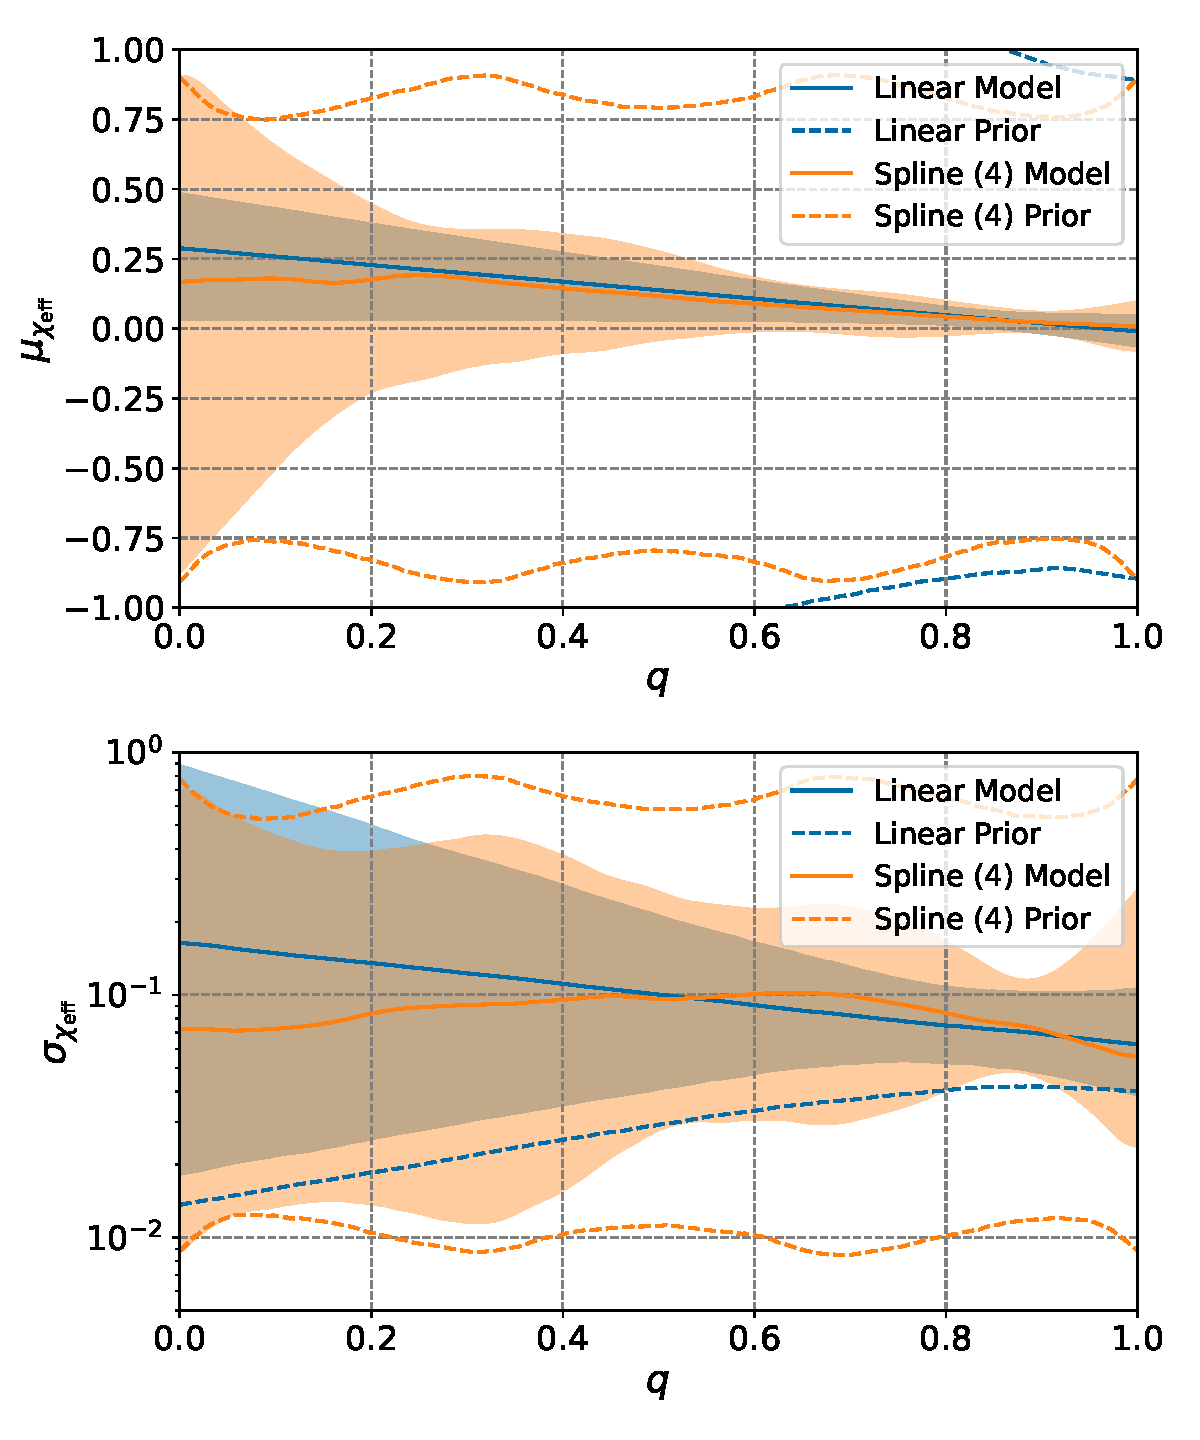
\includegraphics[width=0.9\linewidth]{chieff_q_GWTC3_linear_v_4nodes_unccut.pdf}
    \caption{A comparison between the linear model and 4 node spline model for correlation between $\chieff$ and mass ratio, inferred using \ac{GWTC-3}. Solid lines represent the median, while the shaded region represents the central 90\% credible interval. Dashed lines show the upper and lower boundaries of the prior 90\% interval. The upper panel shows the mean of the $\chieff$ Gaussian as a function of mass ratio $q$, while the lower panel is the standard deviation of the $\chieff$ distribution. For the spline model, the model inference is increasingly prior-driven at small mass ratios, where there is little information in the data.}
    \label{fig:chieff_q_s4_v_linear}
\end{figure}

In Fig. \ref{fig:chieff_q_s4_v_linear}, we show a comparison between our results with the linear model of Ref.~\cite{Callister:2021fpo} to the spline model with 4 nodes. While our spline model results are broadly consistent with the linear model, they generically feature broader credible intervals towards extreme mass ratios $q \to 0$. We argue that this is an advantage of the spline model, as the data should have less information about BBHs with unequal mass ratios as they are less common in the detected population~\cite[e.g.,][]{Fishbach:2019bbm, Farah:2023swu} and be completely uninformative about events with mass ratio $q \to 0$. All of the 69 BBHs in the catalog are inconsistent with vanishing mass ratios, and what's more, our population model with hyperparameter $m_{\rm min} \ge 2\Msun$ (the minimum BH mass must exceed $2\Msun$, see Ref. \cite{Talbot:2018cva}) requires zero support at $q\to0$. Being an approximately local model, the spline model can fit the structure at near-equal mass ratios, while simultaneously saying nothing about the behaviour of extreme mass ratio events. Hence, the posterior approaches the prior as $q\to 0$. We also repeat the analysis with 3-6 nodes and obtain results consistent with the 4-node analysis presented here, see appendix \S \ref{app:extra_analysis}.

To compute the significance of any evolution with mass ratio, we compute the derivative of the inferred evolution with respect to mass ratio. Spline functions are easily differentiable, and so we can compute the slope of the spline function at an arbitrary point $q^*$. We choose the fiducial value of $q^* = 0.9$, as this appears to be a  well constrained region and a good proxy for understanding the evolution of the spin population in the region of near-equal mass ratios. This gives us posteriors on the slope at this point $q^*$ for each model, which we show in Fig. \ref{fig:chieff_q_slope}. We then compute the significance of an evolution in the mean of the Gaussian as a function of mass ratio from the fraction of the posterior support with positive/negative slope. The linear model has a negative slope with significance $\sim 98\%$, as initially reported in Ref. \cite{Callister:2021fpo}. The spline models have negative slope with more inconclusive significance: $\sim 70-80\%$. We show all calculated slope significances at their fiducial values in Table \ref{tab:slope_significance} in appendix \S \ref{app:extra_analysis}. 

We note that this is not the only statistic one could use to quantify the significance. For example, we could consider the difference over widely separated regions in parameter space, e.g. the proportion of samples with mean $\mu(q=1) < \mu(q=0.4)$. These statistics tend to find a similar level of significance.

\begin{figure}
    \centering
    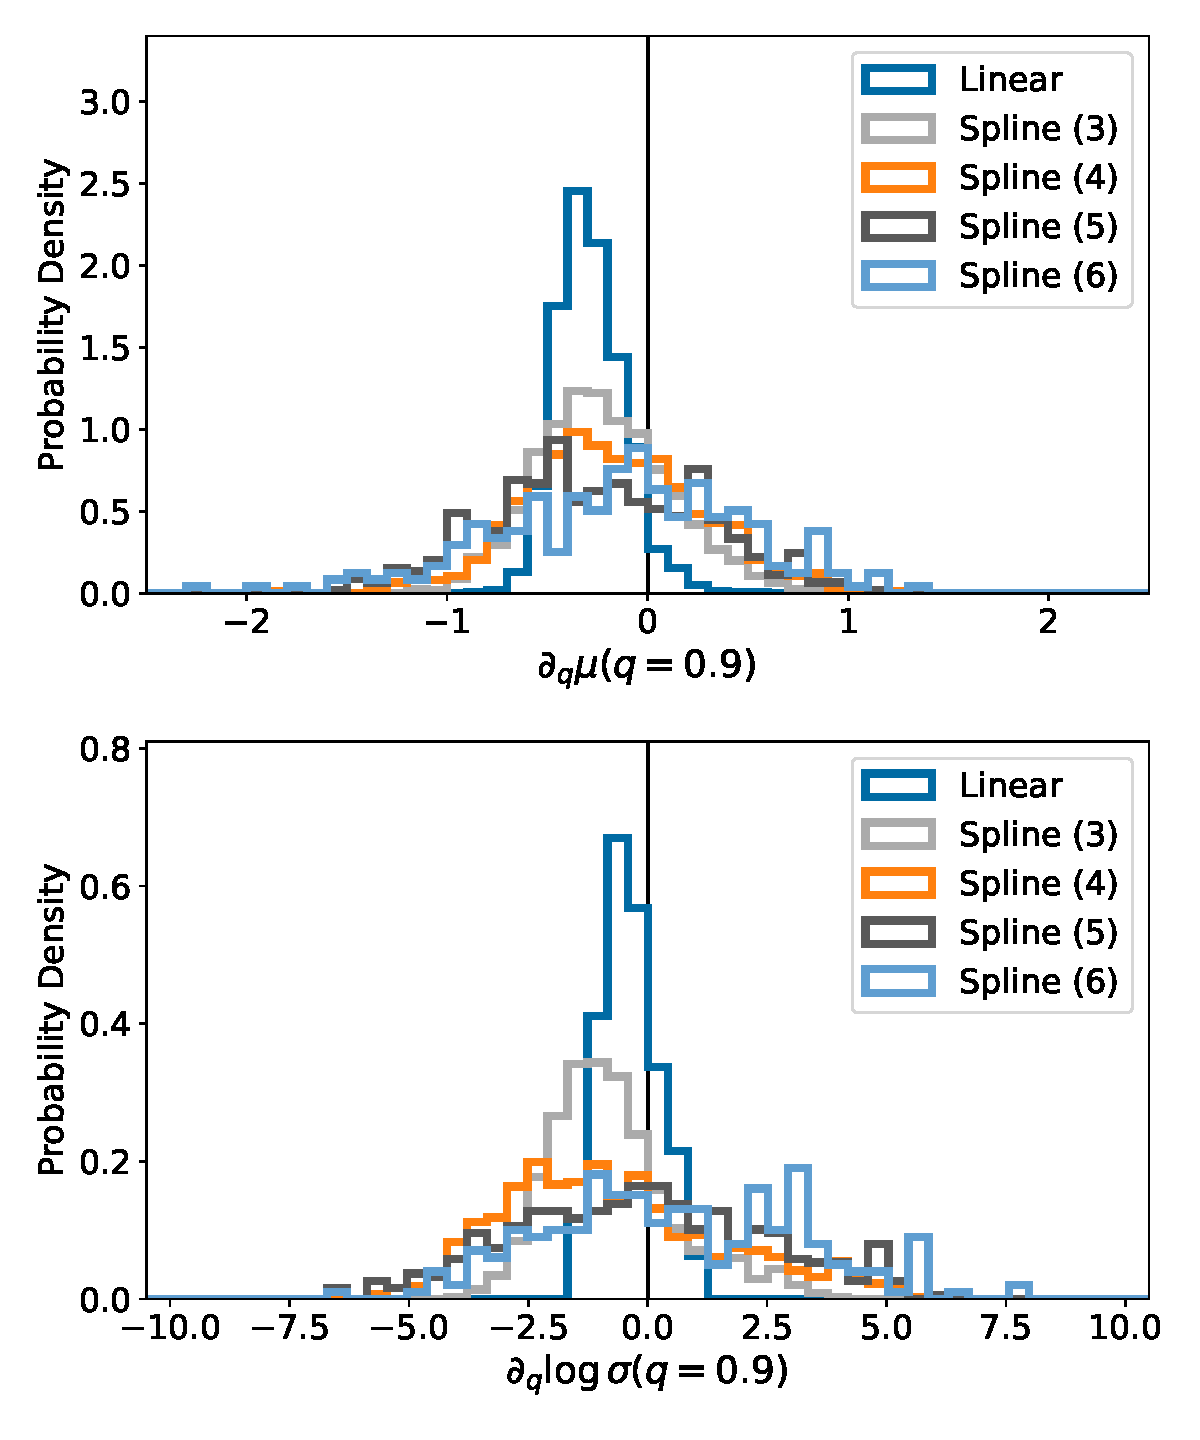
\includegraphics[width=0.9\linewidth]{chieff_q_GWTC3_q0p9_slopes_unccut_1.pdf}
    \caption{Posteriors on the derivative of the mean and width of the $\chieff$ distribution as a function of mass ratio, calculated at $q^* = 0.9$, and inferred using GWTC 3. The linear model concludes that the mean of the $\chieff$ distribution decreases as mass ratio approaches $1$, with a significance of $\sim 98\%$. The spline models are more agnostic, finding significances of $\sim 60-75\%$.}
    \label{fig:chieff_q_slope}
\end{figure}

\subsection{Effective Spin Distribution and Redshift}

Next, we turn our attention to the correlation between $\chieff$ and redshift $z$. Ref.~\cite{Biscoveanu:2022qac} 
examined a correlation between redshift and the effective spin distribution, and discovered evidence for a broadening in the effective spin distribution, a positive correlation between the width $\sigma(z)$ of the $\chieff$ Gaussian and the redshift, and no evidence for any trend in the mean of the Gaussian. In their analysis, Ref.~\cite{Biscoveanu:2022qac} parameterized $\mu(z) = \mu_0 + \delta\mu_z (z-0.5)$ and $\log_{10}\sigma(z) = \log\sigma_0 + \delta\log\sigma_z (z-0.5)$ as linear models and quantified the significance of the measured broadening using the posterior on the slope $\delta\log\sigma_z$.

In a similar approach, we model the $\chieff$ correlation with redshift using Eq. \ref{eq:general_chieff_correlation}, only we use 
\begin{align}
\mu(\theta) &= S\left(z\;|\;(0,\mu_{\chieff:0}), ..., (2.3,\mu_{\chieff:N})\right) \nn \\
\ln \sigma(\theta) &= S\left(z\;|\; (0,\ln \sigma_{\chieff:0}), ..., (2.3,\ln \sigma_{\chieff:N})\right).
\label{eq:chieff_z_spline}
\end{align}
In our model, the first and last nodes are placed at redshifts $z=0$ and $z=2.3$, the maximum redshift we assume in the \pr~model~\footnote{This is somewhat at odds with the maximum redshift considered in the sensitivity injections of~\cite{ligo_scientific_collaboration_and_virgo_2023_7890398}, with $z_{\rm max} = 1.9$. We verified our results are unchanged after considering this adjustment.}. The hyperparameters associated to the splines are the $y$ coordinates of the nodes. We explored models that fix the nodes uniformly between the first and last nodes; however, these resulted in nodes too coarsely spread at small redshift to optimally fit the structure. Additionally, there is limited information in the data thus far to constrain the population much beyond redshift $z \gtrsim 1$, so a better node spacing should place nodes tightly at small redshift and more loosely at high redshift. Heuristically, we found that a linear spacing in $z^{1/2}$ places nodes satisfactorily. 

Using these models to infer the BBH population hyperparameters given the \ac{GWTC-3} dataset, we infer the evolution of the mean and width of the $\chieff$ Gaussian as a function of redshift. We show a comparison between a linear model and the spline model with 4 nodes in Fig. \ref{fig:chieff_z_s4_v_linear}. We show the results for a collection of analyses with 3-6 spline nodes in appendix \S \ref{app:extra_analysis} in Fig. \ref{fig:chieff_correlations} and the associated model evidences in Fig. \ref{fig:chieff_evidences}.

\begin{figure}
    \centering
    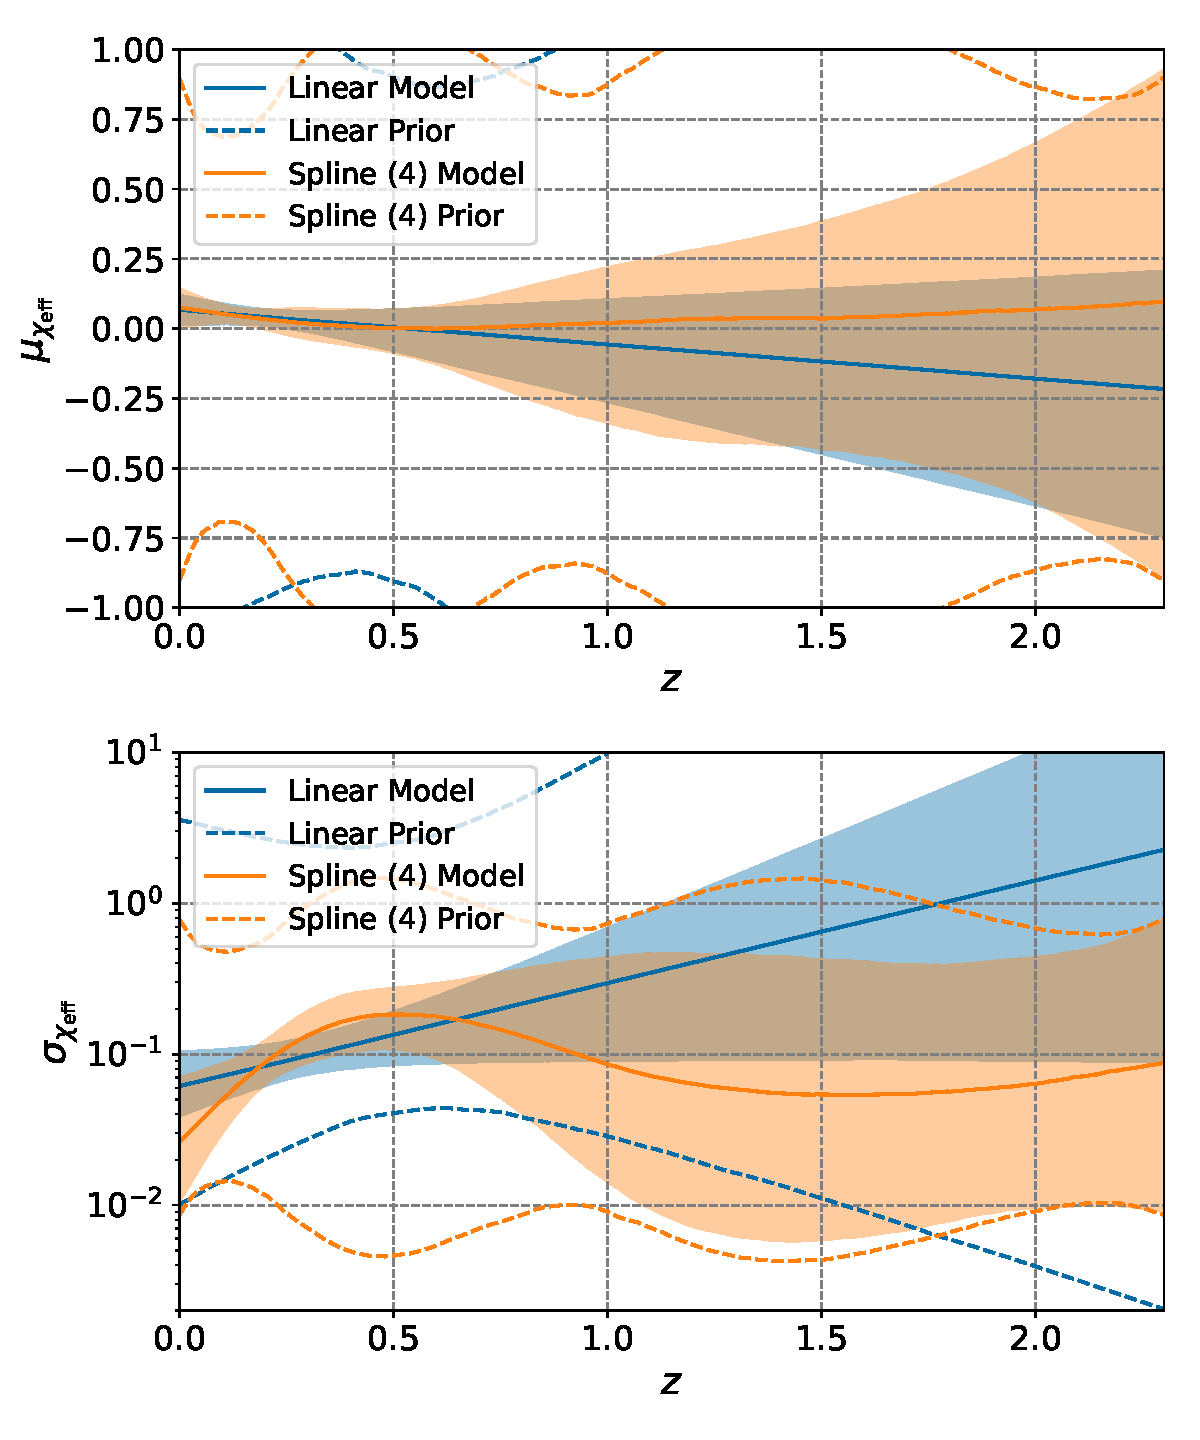
\includegraphics[width=0.9\linewidth]{chieff_z_GWTC3_linear_v_4nodes_unccut.pdf}
    \caption{A comparison between the linear model and 4 node spline model for correlation between $\chieff$ and redshift, inferred using \ac{GWTC-3}. Solid lines represent the median, while the shaded region represents the central 90\% credible interval, and the dashed lines show the boundary of the prior 90\% interval. The upper panel shows the mean of the $\chieff$ Gaussian as a function of redshift $z$, while the lower panel represents the standard deviation of the $\chieff$ distribution. We emphasize that there is very little information in the data at $z \gtrsim 1$, hence the spline inference is prior-driven at these higher redshifts. This is in contrast to the linear model \cite{Biscoveanu:2022qac}.}
    \label{fig:chieff_z_s4_v_linear}
\end{figure}

First, we quantify the confidence of a broadening slope for each model. To this end, we compute the slope of the width of the Gaussian at a fiducial value $z^*$, $\partial \log \sigma(z){z=z^*}$ for all models. 
We choose the fiducial value $z^* = 0.2$ (see appendix \S \ref{app:nonlinear_z} for a discussion on this choice), and show histograms of the slopes for each model in appendix \S \ref{app:nonlinear_z} in Fig. \ref{fig:chieff_z_slope}. We can then quantify the significance of the increase by the proportion of the posterior with slope greater than zero. 

There are varying degrees of evidence that the $\chieff$ distribution is broadening as a function of redshift at $z^*=0.2$, depending on the model used. The mean is decreasing at $\sim 80-95\%$ confidence (the posterior support with slope less than 0), depending on the model assumed. The width is increasing at $90-98.6\%$ confidence, consistent with the finding of Ref.~\cite{Biscoveanu:2022qac} that the width of the $\chieff$ distribution broadens with increasing redshift. We collect all significances calculated at fiducial values in Table \ref{tab:slope_significance} in appendix \S \ref{app:extra_analysis}.

\begin{figure*}
    \centering
    % 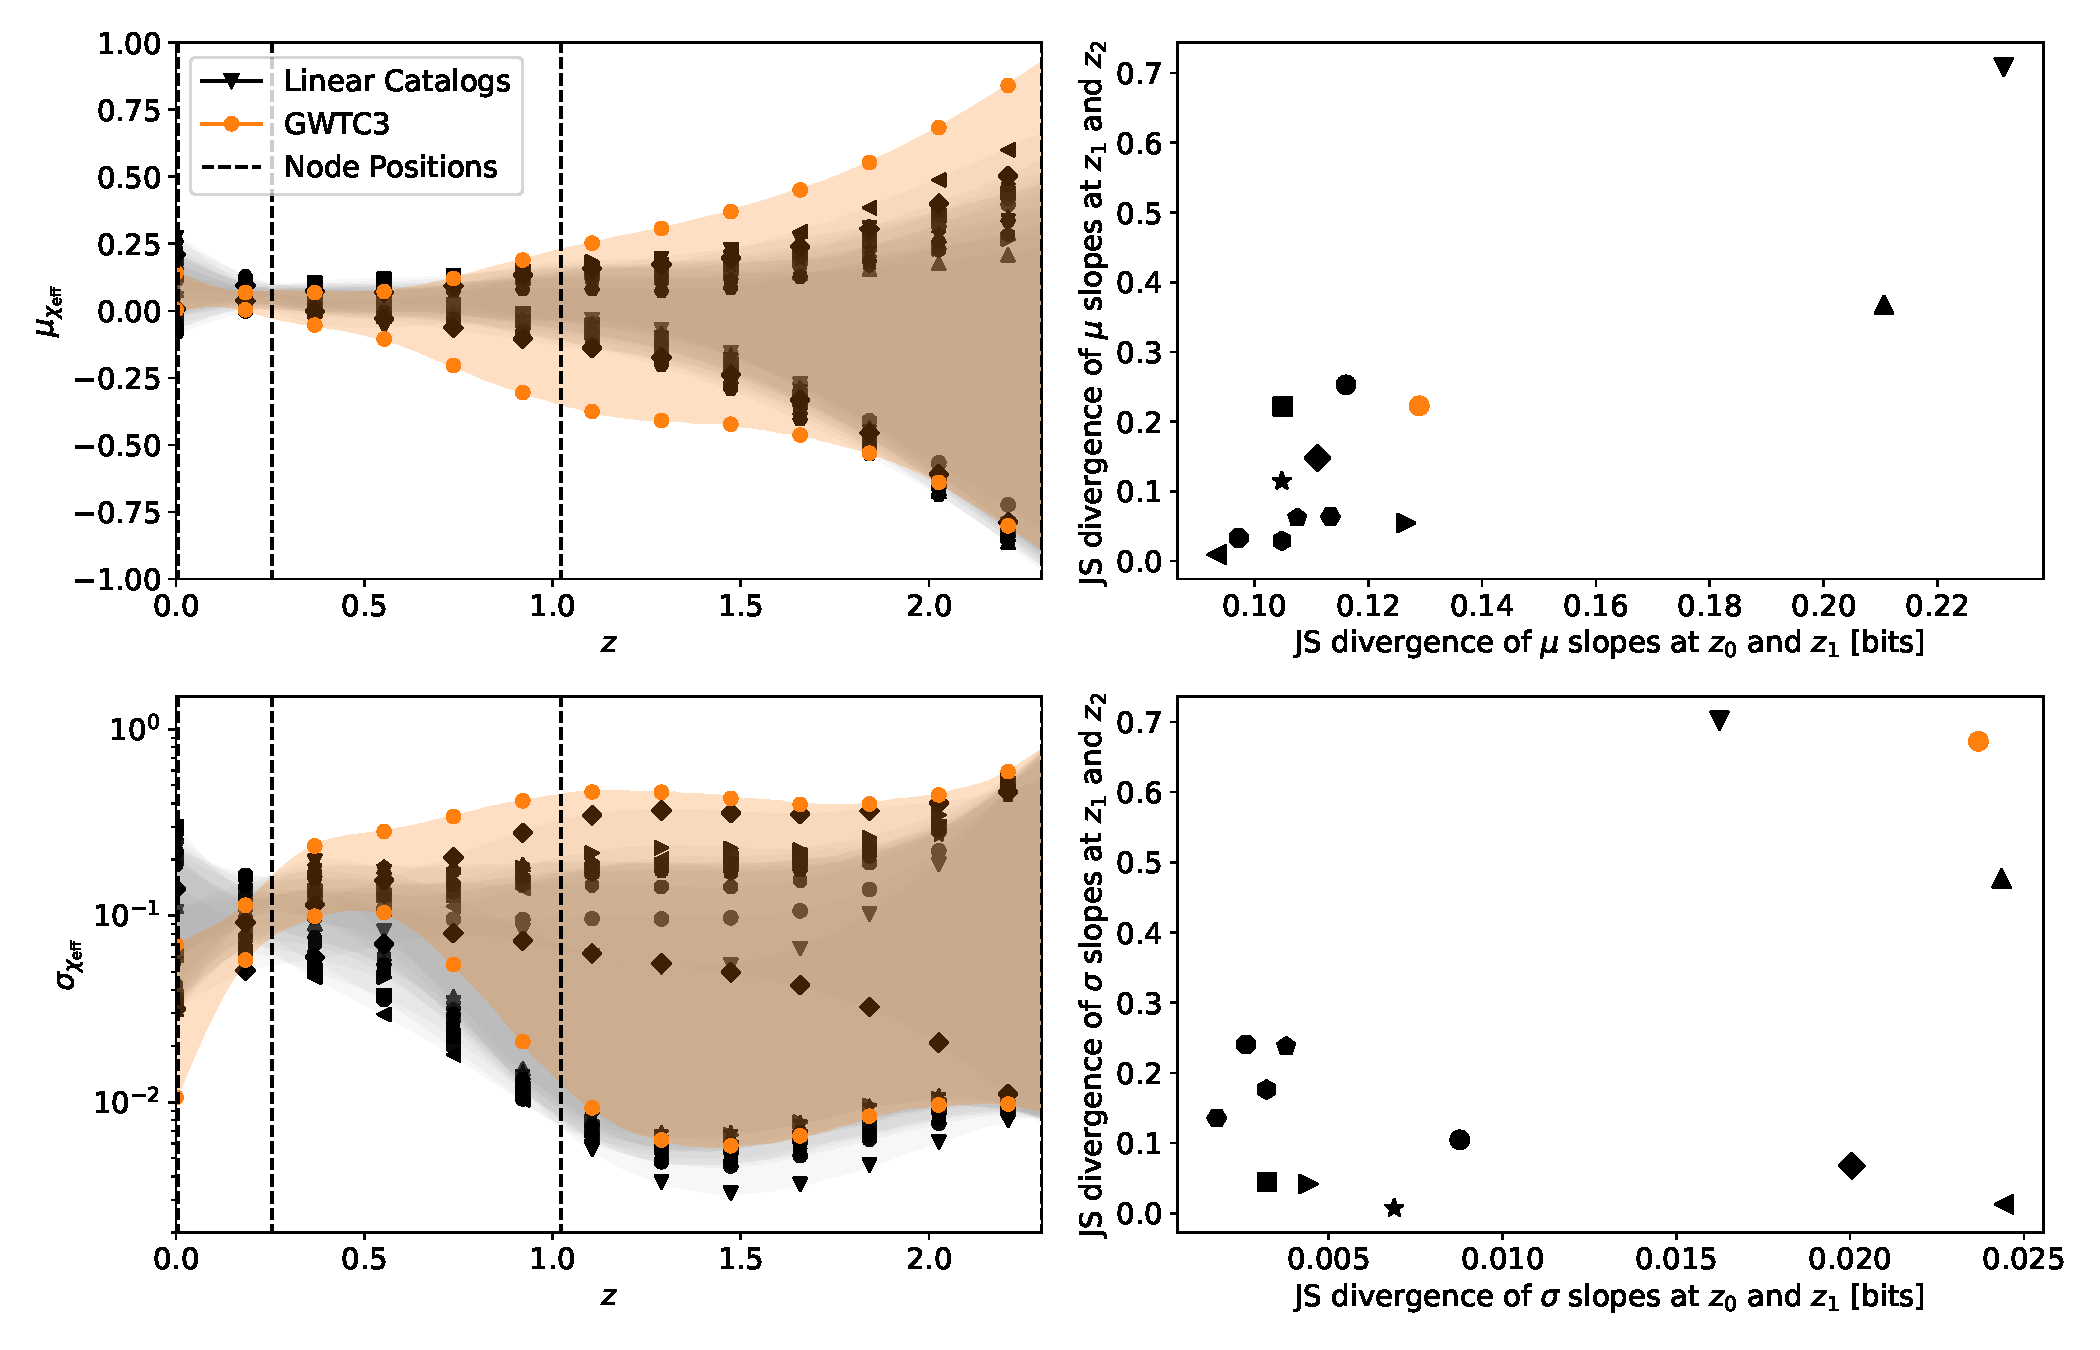
\includegraphics[width=0.9\linewidth]{chieff_z_comparison_plot_linear_v_gwtc3_JS_evenMarkers.pdf}
    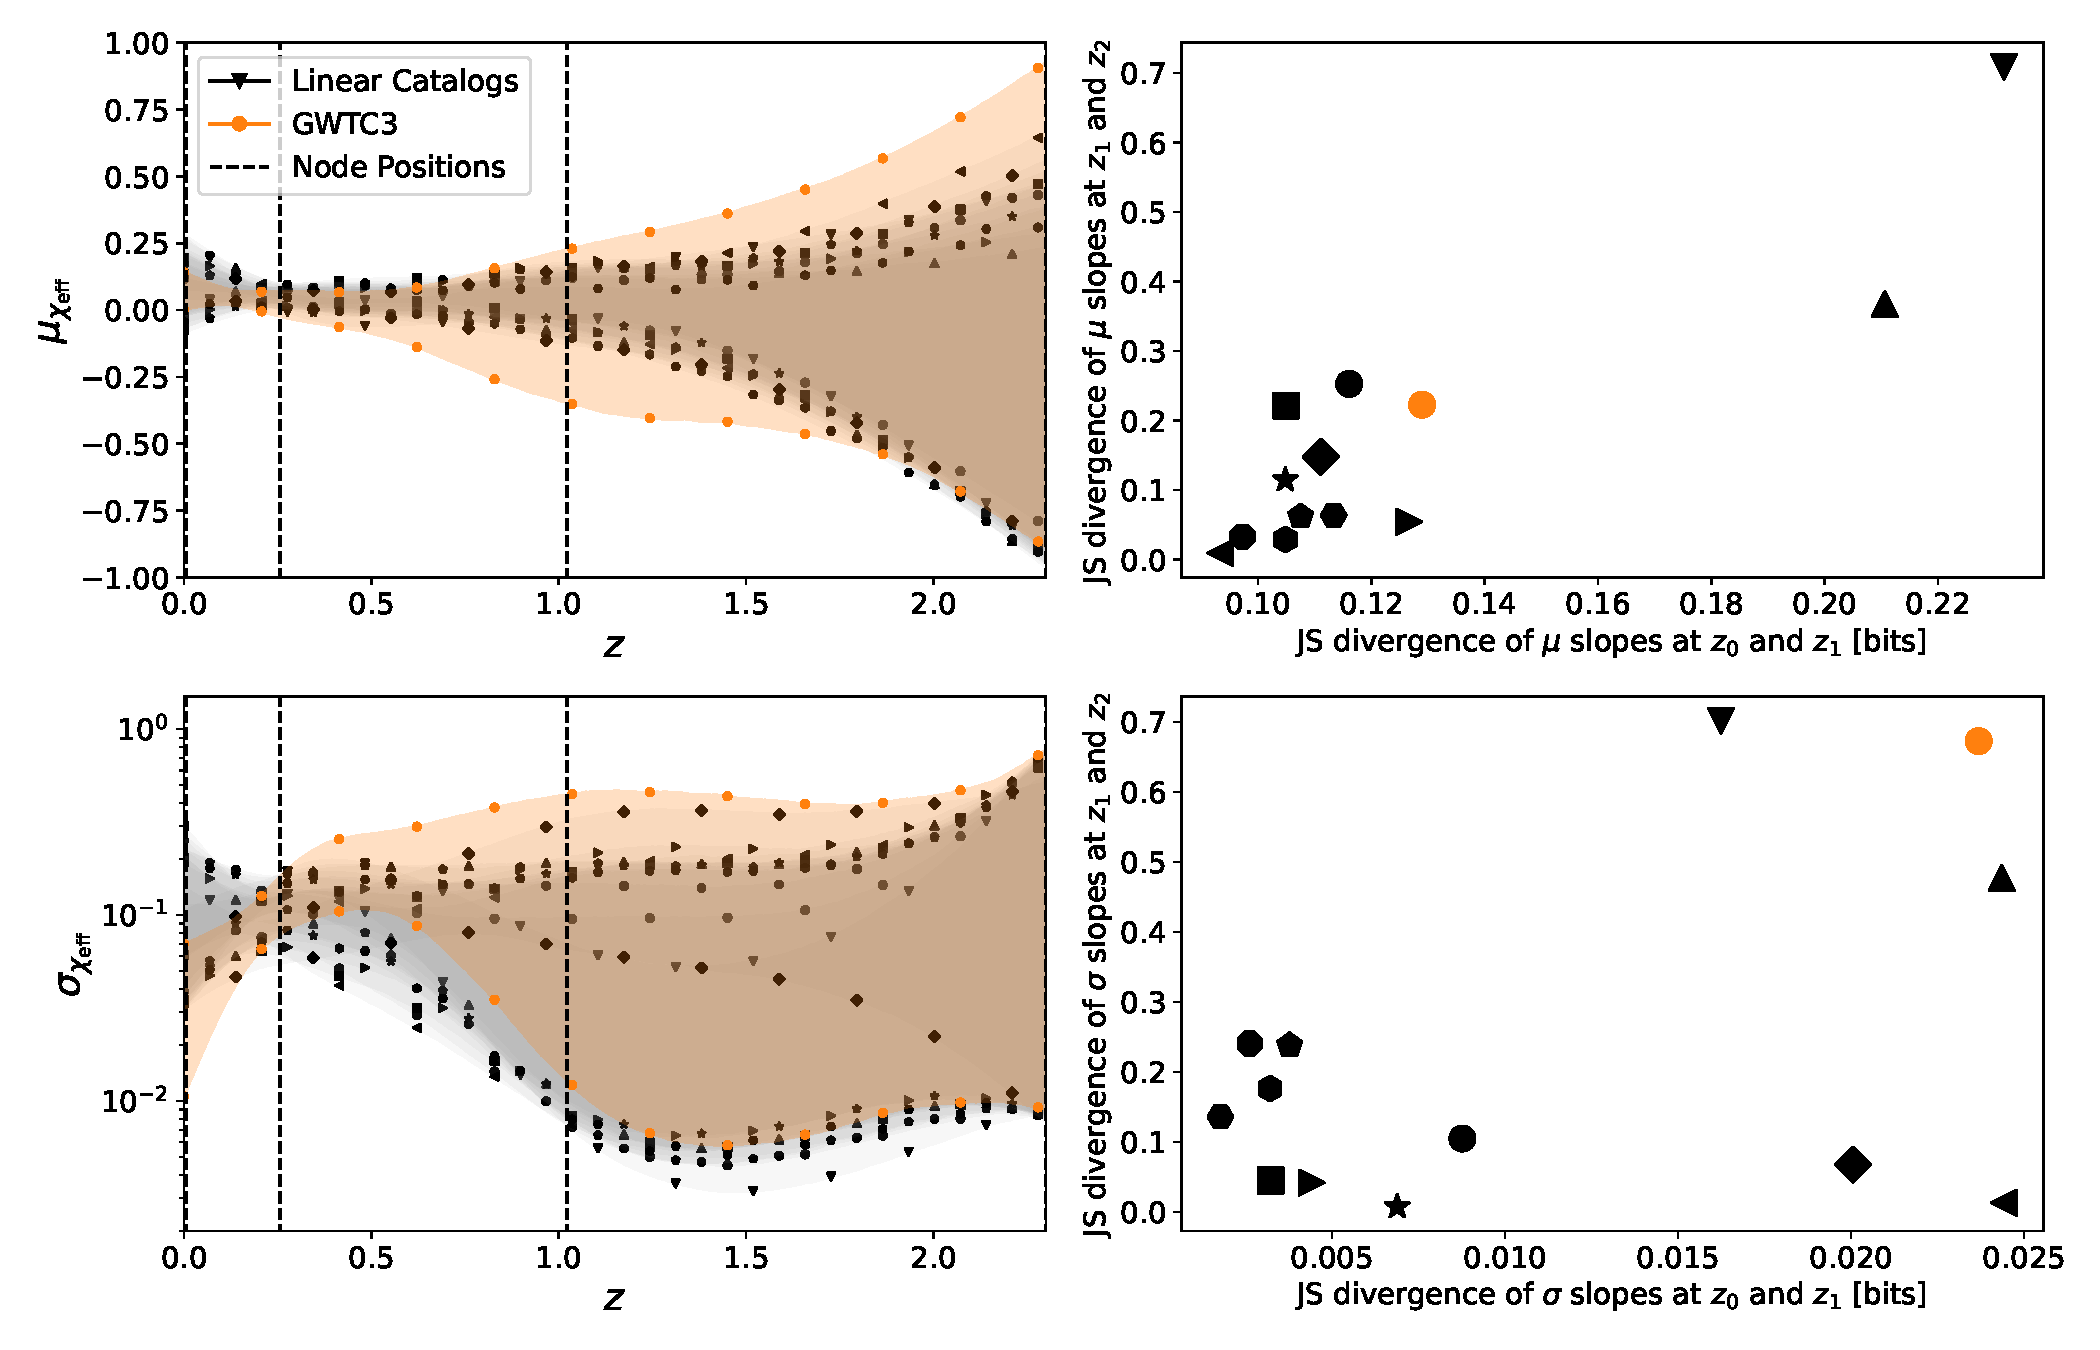
\includegraphics[width=0.9\linewidth]{chieff_z_comparison_plot_linear_v_gwtc3_JS_shiftedMarkers.pdf}
    % \includegraphics[width=0.9\linewidth]{chieff_z_comparison_plot_linear_v_gwtc3_JS.pdf}
    % the commented out plot shifts each marker, but I (Jack) thought it looked uglier actually,
    \caption{Comparison between the spline inference on a linearly correlated Universe and the inference on \ac{GWTC-3}. The first row shows the mean and the second row the standard deviation. The left column shows the 90\% credible intervals inferred using \ac{GWTC-3} (orange) and the 12 synthetic catalogs of 69 events drawn from a linearly correlated Universe (gray). The right column shows the \acf{JS} divergences (in bits) between slope posteriors taken at the first two nodes on the x-axis, and between the second and third nodes on the y-axis. For each linear catalog there is a black point on the scatter plot, and the orange point corresponds to the \ac{GWTC-3} divergences. This represents the posterior difference between the two slopes, quantifying the nonlinearity. The further the point is from the origin, the more confident we are in the inferred nonlinearity. Notice there is no inference on a linear Universe which is more nonlinear than \ac{GWTC-3} in both dimensions.}
    \label{fig:nonlinearity_quantification}
\end{figure*}

It also appears that there is some nonlinearity in the evolution of the width as a function of redshift. To understand if this degree of inferred nonlinearity is expected in a Universe with a linear correlation, we perform the spline model inference with 4 nodes on 12 catalogs of 69 events drawn from a linearly correlated Universe, (see appendix \S \ref{app:nonlinear_z} for details on the selection procedure and the generation of the synthetic catalogs). We then compute the derivative at the first three nodes $z_0$, $z_1$ and $z_2$ (ignoring the last node since the posterior is essentially the prior there) and calculate the \acf{JS} divergence~\cite{kullback1951, Lin:1991zzm} between the slope posteriors. A linearly correlated Universe would theoretically have slope posteriors all consistent with the true value, however there will be some random scatter between the posteriors, measured by the \ac{JS} divergence between them. Looking at a scatter plot of the divergence between the slope at $z_0$ and $z_1$ on the x-axis and between $z_1$ and $z_2$ on the y-axis in Fig. \ref{fig:nonlinearity_quantification}, notice that there are no divergences from a linearly correlated Universe which is more extreme than the \ac{GWTC-3} divergences in both axes. This points towards a nonlinear trend in the width of the $\chieff$ distribution as a function of redshift, though the Bayesian evidence ($\mathcal{Z} = \int \pi(\Lambda) \mathcal{L}(\{d_i\}|\Lambda) d\Lambda$) is not yet conclusive (see Fig. \ref{fig:chieff_evidences} in appendix \S \ref{app:extra_analysis})


% \subsection{Simultaneous Inference: Which Parameter(s) Correlate?}

% Above, we have considered each correlation separately, assuming that only one parameter may correlate at a time. Further, one might worry about a false inference of a spin correlation with one parameter due to a different confounding correlation with another parameter. This problem appears by inferring with a potentially wrong hypothesis, hence we introduce a more general hypothesis which allows for a correlation with any parameter.
% Finally, we introduce a model which combines Eqs. \ref{eq:chieff_q_spline}, \ref{eq:chieff_z_spline} and \ref{eq:chieff_m_spline} in a mixture model to understand which parameter correlation is preferred by the data, or if some combination is preferred. In particular, we use the model


% Dirichlet model... way too expensive never finishes... maybe run with a bunch of cores...

\section{Future Prospects: Can We Detect Nonlinearity in O4?}
\label{sec: spline o4_projections}
Flexible spline models stand in contrast to linear models, where the correlation around each spline node is independently inferred, rather than enforcing a consistent slope across the whole parameter space. 
%bona-fide constraints in one region of parameter space may lead to erroneous constraints elsewhere. 
At the conclusion of O3, these flexible models highlight our lack of knowledge about poorly constrained regions. While we have some hints of a nonlinear correlation in $\chieff-z$, there is not yet a definitive preference in the Bayesian evidence for a nonlinear correlation. This may change by the end of the fourth observing run, O4. 

To predict how well we may actually detect nonlinear correlations in the future, we produced two synthetic catalogs of 200 events and 400 events for two different possible Universes (so four catalogs total). The events are detected by a network of LIGO interferometers (located at Hanford and Livingston), assuming the fiducial O4 noise spectra with an average BNS inspiral range of 160 Mpc~\cite{O3_psds}. We draw \ac{GW} events from a few different populations with true hyperparameters given in Table \ref{tab:true_hyper}. These populations are consistent with the data collected by the \ac{LVK} thus far, analyzed with the models we presented above. We use the waveform model \texttt{IMRPhenomXP} with \texttt{PrecVersion=104}~\cite{Pratten:2020ceb}, and use the heterodyning/relative binning scheme of Refs.~\cite{Cornish:2010kf, Cornish:2021lje, Zackay:2018qdy} to efficiently sample the \ac{GW} event parameter posteriors.

\renewcommand{\arraystretch}{1.25}
\begin{table*}
    \centering
    \resizebox{\textwidth}{!}{
    \begin{tabular}{|l||lll|}
       \hline Hyperparameter & Description & $q-\chieff$ Correlation & $z-\chieff$ Correlation \\
       \hline $\alpha$ & $m_1$ power-law index & $3$ & $3$ \\
       $\beta$ & $q$ power-law index & 1 & 1 \\
       $m_{\rm max}$ & maximum BH mass & $85\Msun$ & $85 \Msun$ \\
       $m_{\rm min}$ & minimum BH mass & $5\Msun$ & $5 \Msun$ \\
       $\delta_m$ & low-mass smoothing parameter & $3\Msun$ & $3\Msun$ \\
       $\mu_{m}$ & $m_1$ Gaussian component mean & $35\Msun$ & $35 \Msun$ \\
       $\sigma_{m}$ & $m_1$ Gaussian component standard deviation  & $5\Msun$ & $5\Msun$ \\
       $\lambda$ & fraction of BBHs in Gaussian component & $0.03$ & $0.03$ \\
       $\lambda_z$ & $z$ power-law index & 2 & 2 \\ \hline
       $(x_0, \mu_{\chieff:0})$ & first mean spline node coordinates & $(0, 0.4)$ & $(0, 0)$ \\
       $(x_1, \mu_{\chieff:1})$ & second mean spline node coordinates & $(0.4, 0.3)$ & $(0.3, 0)$ \\
       $(x_2, \mu_{\chieff:2})$ & third mean spline node coordinates & $(0.8, 0.05)$ & $(0.65, 0)$ \\
       $(x_3, \mu_{\chieff:3})$ & fourth mean spline node coordinates & $(1, 0.02)$ & $(2.3, 0)$ \\
       $(x_0, \ln\sigma_{\chieff:0})$ & first standard deviation spline node coordinates & $(0, -2.5)$ & $(0, -3.5)$ \\
       $(x_1, \ln\sigma_{\chieff:1})$ & second standard deviation spline node coordinates & $(0.4, -2.5)$ & $(0.3, -2)$ \\
       $(x_2, \ln\sigma_{\chieff:2})$ & third standard deviation spline node coordinates & $(0.8, -2.5)$ & $(0.65, -1.5)$ \\
       $(x_3, \ln\sigma_{\chieff:3})$ & fourth standard deviation spline node coordinates & $(1, -2.5)$ & $(2.3, -1.25)$ \\ \hline
    \end{tabular}}
    \caption{Hyperparameters for the simulated Universes with nonlinear correlation. In the left column are the hyperparameters for the Universe with a correlation between $\chieff$ and mass ratio, and in the right column is the correlation with redshift. The correlation functions are themselves splines, with node placements given by e.g. the $(z_N, \mu_{\chieff:N})$ coordinate pairs.}
    \label{tab:true_hyper}
\end{table*}

We then select detected events on a network matched-filter SNR $\rho_{\rm mf, HL} > 9$, and generate a set of Monte Carlo injections for estimating the selection efficiency consistent with this detection criterion \cite{Essick:2023toz}. This kind of selection criterion implicitly depends on the true binary system parameters, which is not a physical assumption \footnote{There is an issue here with nomenclature. Often, the matched-filter SNR is defined as a \textit{maximization} over a fixed signal bank, however for synthetic catalogs it is typical to compute the matched-filter SNR with the signal from the true source parameters. These statistics are conditioned on different things: the former is conditioned only on the data, because the signal bank is fixed, while the latter is conditioned on the data \textit{and} the true signal parameters.}. This means that the hierarchical likelihood of Eq. 3 should be slightly modified to match this different selection criterion. However, we use the same likelihood of Eq. 3 as an approximation. he bias is likely small for catalogs of relatively small size, such as the ones in this work, but it should be noted that this may be present in our inferences on synthetic catalogs \cite{Essick:2023upv}.

We recover each simulated catalog assuming both a linear model and the spline model with 4 nodes. We restrict to one spline analysis using 4 nodes to limit the computational expense. 

We decided to explore two node placement options. First, we recover using our original node placement scheme, placed in the same manner as described above (linear in $q$ and $z^{1/2}$). This node placement does not match the true node placement (Table \ref{tab:true_hyper}), and the inference finds more ``bumps'' in the correlation than are truly there. To this end, we also recover using the true node placement scheme. See appendix \S \ref{app:node_placement_bias} for a discussion on node placement and bias in the inference.

% Splines are flexible enough for recovering general nonlinear functions; however they are notorious for finding spurious structure~\cite[e.g.,][]{Farah:2023vsc}. % Indeed, our results on these mock catalogs reiterate the sensitivity of spline model results on node placement and the skepticism with which one should interpret spline constraints. \rednote{Where is the right balance between yes, splines are wiggly, but don't throw away our paper?}

We show our results comparing the linear model and the spline model with our original node placement (linear in $q$ and $z^{1/2}$) in Fig. \ref{fig:chieff_q_mock_catalog_s4_v_linear}.
\begin{figure}
    \centering
    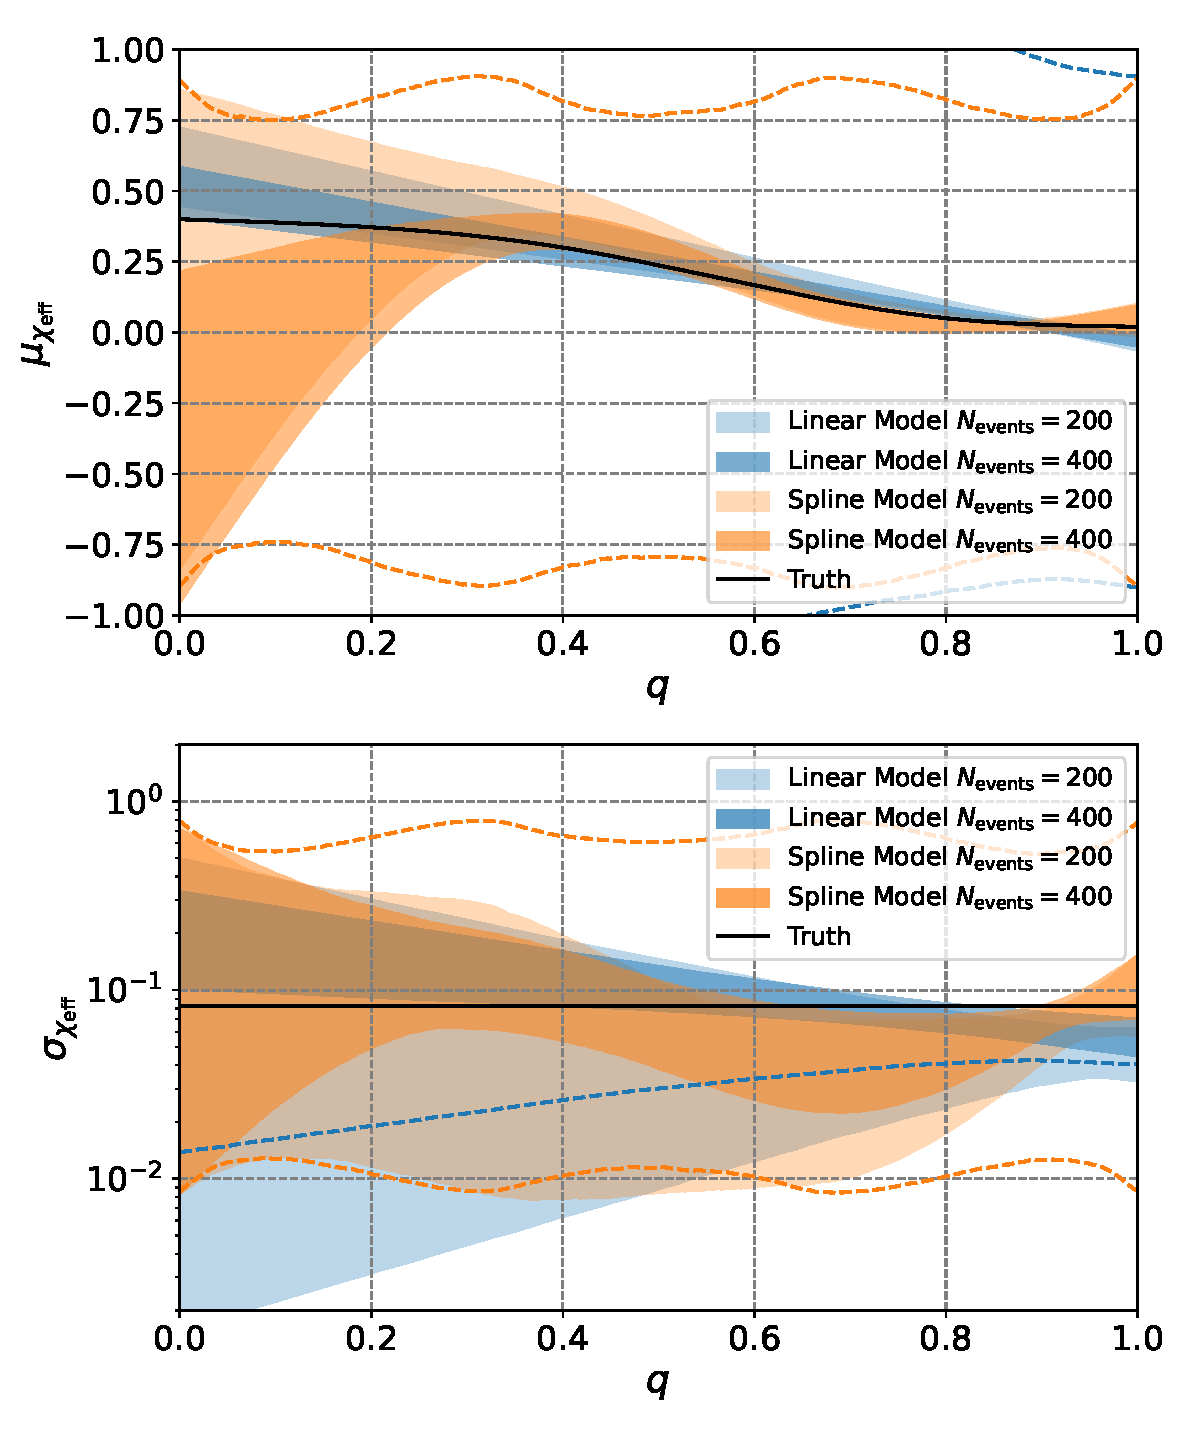
\includegraphics[width=0.9\linewidth]{mock_catalogs_chieff_q_GWTC3_q_linear_v_4nodes.pdf}
    \caption{Inferred mean and width of the $\chieff$ distribution as a function of mass ratio $q$ on two mock catalogs. In blue are the 90\% credible intervals when assuming a linear model for the correlation, while in orange are the 90\% intervals inferred under the spline model with 4 nodes. The lighter shades represent the inference on a catalog with 200 events, while the darker shade is with 400 events. Dashed lines represent the prior 90\% region, and in solid black is the true correlation.}
    \label{fig:chieff_q_mock_catalog_s4_v_linear}
\end{figure}

In a catalog of 200 detections, the model evidences indicate no significant preference for a linear model or the spline model. Indeed, the Bayes factor of the spline model over the linear model with 200 events is $\log_{\rm 10}\mathcal{B}_{s|l}(200) = 0.00 \pm 0.13$. However, when we increase the number of detections to 400, the data begins to indicate a slight preference for the spline model, although nothing yet conclusive; $\log_{\rm 10}\mathcal{B}_{s|l}(400) = 0.28 \pm 0.14$. We emphasize that this holds for a particular choice of a nonlinear correlation. In truth, the correlation may be more or less linear than the one we simulated, which would make evidence of nonlinearity correspondingly more or less definitive at these numbers of events. 


\begin{figure}
    \centering
    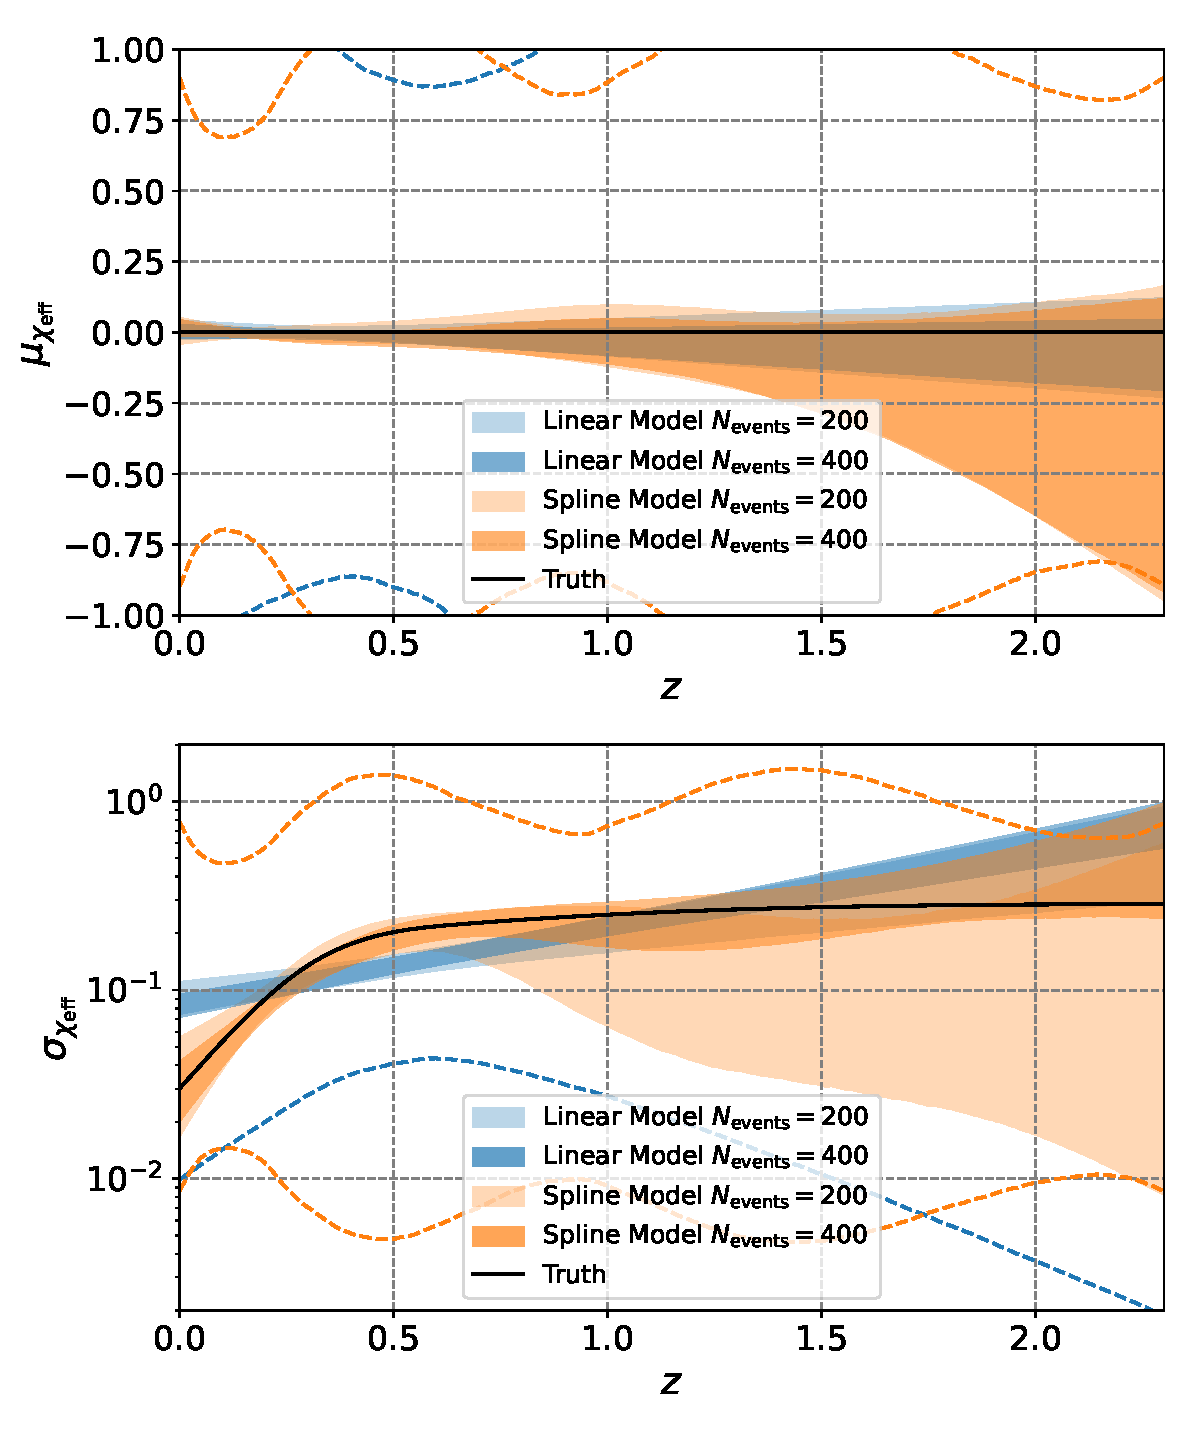
\includegraphics[width=0.9\linewidth]{mock_catalogs_chieff_z_GWTC3_z_linear_v_4nodes.pdf}
    \caption{Inferred mean and width of the $\chieff$ distribution as a function of redshift $z$ on two mock catalogs. In blue are the 90\% credible intervals when assuming a linear model for the correlation, while in orange are the 90\% intervals inferred under the spline model with 4 nodes. The lighter shades are the inference using a catalog of 200 events, while the darker shade is with 400 events. Dashed lines represent the prior 90\% region, and in solid black is the true correlation.}
    \label{fig:chieff_z_mock_catalog_s4_v_linear}
\end{figure}


To understand how we may constrain the correlation between the spin population and the redshift in the future, we also simulated a Universe with a nonlinear correlation between the width of the $\chieff$ distribution and redshift (see Table \ref{tab:true_hyper}), where the model hyperparameters chosen are consistent with the catalog through the end of the third observing run. 

We once again produced mock catalogs with 200 and 400 detections, and we show the results of the inferences in Fig. \ref{fig:chieff_z_mock_catalog_s4_v_linear}. This time, even a false node placement scheme does a good job at fitting the correlation. Furthermore, model evidences become conclusively in favor of the nonlinear model with a catalog of 400 detections. In particular, for the redshift correlation $\log_{\rm 10}\mathcal{B}_{s|l}(200) = 1.06 \pm 0.14$ and $\log_{\rm 10}\mathcal{B}_{s|l}(400) = 4.09 \pm 0.16$.
We also checked that a spline model with nodes placed in the correct locations produce consistent results, as expected.

We reiterate that the results of this projection study depend on the assumed true correlation. However, since the correlation we chose is consistent with the data collected thus far, this demonstrates that we \textit{can} detect nonlinearity in the spin correlation with a catalog of $\sim400$ detections. 

\section{Conclusions}
\label{sec: spline conclusion}
In this paper we presented a flexible model for understanding the correlation between the spin population in $\chieff$ and primary mass $m_1$, mass ratio $q$ or redshift $z$. On the \ac{LVK} data published thus far, we obtain results broadly consistent with previous analyses \cite{Safarzadeh:2020mlb,Callister:2021fpo,KAGRA:2021duu,Biscoveanu:2022qac,Franciolini:2022iaa}. Furthermore, because of their flexibility, these spline models highlight the regions of parameter space that drive a measured correlation, and the regions of parameter space which are more uncertain. %, with some potential improved constraints on the correlation with redshift and the correlation with primary mass. 

In particular, we find that the mean of the $\chieff$ distribution likely increases with mass ratio, the width likely broadens with redshift, and may also broaden for more massive binaries. Importantly, it is also possible that not all of these claims are true at the same time. Perhaps a correlation with one parameter may masquerade as a correlation with another parameter when analyzed under the false hypothesis. Ref. \cite{Biscoveanu:2022qac} studied this possibility using linear models which simultaneously fit the correlation with $m$, $q$ and $z$, and found that the data is not yet informative enough to answer this question, though it appears possible that all correlations are real. While we do not consider simultaneous models in this work, we do observe the Bayes factors all appear consistent, suggesting the data is not yet informative enough to pick out any mismodeled correlations.
 
%Without further analysis, it is impossible to determine which correlations are truly bona-fide and which (if any) are simply artifacts of an analysis under a false hypothesis. A future analysis may be able to let the data inform us which correlation(s) are truly present. 

Each of these potential correlations may prove to be important probes of the astrophysical environments which produce BBHs. The observed anticorrelation between the mean of the $\chieff$ distribution with mass ratio may indicate that the BBHs observed come from binaries which experience mass ratio reversal using an optimistic common envelope (CE) prescription \cite{Broekgaarden:2022nst}, or isolated binaries which either undergo a CE phase with large CE efficiency or stable mass transfer with super-Eddington accretion \cite{Bavera:2020uch, Zevin:2022wrw}. It is also possible that hierarchical mergers in a dense environment can produce the observed correlation; we would expect hierarchical mergers involving just one second-generation black hole from a previous merger to have more extreme mass ratios and higher spins~\cite[e.g.,][]{Gerosa:2021mno}. However, in an environment with isotropic spin symmetry, the $\chieff$ distribution must be centered on zero, and so one would expect a \textit{broadening} of the distribution at small mass ratios, not an increase in the mean. In order to produce the observed correlation, then, the environment must break isotropy symmetry somehow \cite{Santini:2023ukl}, e.g., in an AGN disk \cite{McKernan:2021nwk, Santini:2023ukl}. Finally, if the observed BBHs do not originate from one channnel, but a superposition of multiple \cite[e.g.,][]{Zevin:2020gbd,Cheng:2023ddt}, a (linear) correlation may arise from a Simpson's-type paradox, where multiple populations naturally separated in $\chieff-q$ space are % incorrectly
interpreted as a correlation \cite{Baibhav:2022qxm}. Especially in this last scenario, a flexible nonlinear model will help shed light on the origin of the $\chieff-q$ correlation as we move into O4. 

The correlation with redshift probes evidence for other kinds of pathways toward merging stellar mass BBHs. This observation is commonly explained by connecting the spin-up of a BH or its progenitor with the delay time to merger. If the spin-up mechanism of BH progenitors is stronger for closer separations, the remnant \ac{BBH} system will radiate energy to GWs more rapidly, and hence merge earlier. Because \acp{BBH} are born at a higher rate at higher redshifts, this results in a positive correlation between spin magnitude and redshift \cite{Zaldarriaga:2017qkw,Bavera:2020inc,Bavera:2021evk,Fuller:2022ysb}. One potential mechanism is tidal torques: the spin-up due to tidal torques is amplified if the binary is at a smaller initial separation. If the stellar progenitors retain some angular momentum upon collapse, the BH spins should be correlated with the observed redshift at merger \cite{Qin:2018vaa, Fuller:2019sxi, Bavera:2022mef}. This is complicated by the expectation that formation in the field produces nearly aligned spins. In this scenario, then there should be a positive correlation between redshift and the mean of the Gaussian; increasing the width requires larger spins with a more isotropic tilt distribution. If there are strong supernova kicks, however, this can even out the spin tilts and give a $\chieff$ distribution more centered on zero \cite{Rodriguez:2016vmx, Gerosa:2018wbw, Callister:2020vyz, Stevenson:2022hmi}.

Finally, a correlation between $\chieff$ and the primary mass is most naturally understood as a signature of hierarchical mergers. In this paper, we observe a broadening of the $\chieff$ distribution as the primary mass increases, with varying levels of confidence depending on the model (see appendix \S \ref{app:chieff_m}). This is precisely the expectation of a hierarchical merger picture in an environment endowed with isotropy symmetry \cite{Gerosa:2021mno, Gerosa:2017kvu, Fishbach:2017dwv, Tagawa:2021ofj}. That said, the most recent studies which directly searched for signatures of hierarchical mergers in the \ac{LVK} catalog strongly disfavor scenarios where all the \ac{LVK} BBHs are formed hierarchically \cite{Fishbach:2022lzq, Doctor:2019ruh, Kimball:2020opk}, though they cannot be ruled out as a subpopulation.

To understand how we might probe nonlinear correlations in the future, we also simulated nonlinearly correlated Universes consistent with the data collected thus far. In a Universe with a nonlinear correlation between $\chieff$ and mass ratio, we found that a linear model may still be appropriate with $\sim 400$ detections, although this is of course heavily dependent on how nonlinear the true correlation is. For a nonlinear correlation in the $z-\chieff$ plane, we find that a linear model may be significantly disfavored as we approach $\sim 400$ detections. Because the nonlinear correlations we assumed were consistent with \ac{LVK} data collected thus far, it is possible that linear models for correlation will begin to fail by the end of O4. 

However, we also encountered a few drawbacks with spline functions. For one, flexible models are intrinsically high dimensional, and thus sampling from the hyperposterior can become significantly more expensive. Second, spline models are perhaps too good at finding nonlinearities, to the point of confidently finding nonlinear features even when they are not present (see appendix \S \ref{app:node_placement_bias}). To be confident in a spline-feature, one should recover the feature varying the number of nodes or the locations of the nodes, or even directly estimate the false alarm probability as in Ref.~\cite{Farah:2023vsc}.

In this paper, we argue that flexible models for correlation offer a complementary but equally important perspective compared to strongly parameterized models. Foremost, spline models can effectively fit a much wider range of potential correlations. We do not \textit{a-priori} expect nature to provide us with linear correlations, or even correlations that can be well-approximated by a line~\cite[e.g.,][]{Belczynski:2017gds, PortegiesZwart:2002iks, Rodriguez:2015oxa, Gerosa:2021mno}.  The correlations in nature may be strongly nonlinear, or perhaps form as a result of a superposition of subpopulations, and these can only be observed when analyzed with a sufficiently flexible model. Of course, it is possible the correlations will indeed turn out to be linear, however we can only observe such a phenomenon by allowing for the alternative.


% As we demonstrated in this paper, a simple and effective method for searching for nonlinear correlations is to parameterize the correlation as a cubic spline function. 



% Taking the pros and cons together, then, the right approach should require a healthy dose of skepticism to accompany any claim based entirely on a spline model. That is not to say they are not useful. On the contrary, spline models are a simple way of searching for candidate structures across parameter space. To be confirmed or discarded, any candidates must be followed up with a subsequent study, perhaps by using a more direct parameterization, or by directly estimating the false alarm probability \cite{Farah:2023vsc}. \rednote{lighten it up a bit!}


\section{Acknowledgements}

We thank Tom Callister, Matthew Mould, and Colm Talbot for helpful suggestions and relevant expertise. We thank Christian Adamcewicz for reviewing this work during LVK interval document review and for providing helpful comments. We also thank the anonymous referee for the helpful suggestions.
This material is based upon work supported by NSF's LIGO Laboratory which is a major facility fully funded by the National Science Foundation. LIGO was constructed by the California Institute of Technology and Massachusetts Institute of Technology with funding from the National Science Foundation and operates under cooperative agreement PHY-0757058. J.H. and S.B. are supported by the NSF Graduate Research Fellowship under Grant No. DGE-1122374. S.B. is also supported by NASA through the NASA Hubble Fellowship grant HST-HF2-51524.001-A awarded by the Space Telescope Science Institute, which is operated by the Association of Universities for Research in Astronomy, Inc., for NASA, under contract NAS5-26555.
S.V. is also supported by NSF PHY-2045740. The authors are grateful for computational resources provided by the Caltech LIGO Laboratory and supported by NSF PHY-0757058 and PHY-0823459.

%\bibliography{main}  % commented out — global biblatex handles bibliography

\section{Appendix}

\subsection{Effective Spin Distribution and Primary Mass}
\label{app:chieff_m}

We also search for potential correlation in the population between the $\chieff$ distribution and the primary mass $m_1$. Previous studies have searched for the same correlation (see, e.g., Refs. \cite{Safarzadeh:2020mlb,Biscoveanu:2022qac}) using a linear model for the mean and width in Eq. \ref{eq:general_chieff_correlation}, and discovered weak evidence for a trend in the width of the $\chieff$ distribution. 

\begin{figure}[h!]
    \centering
    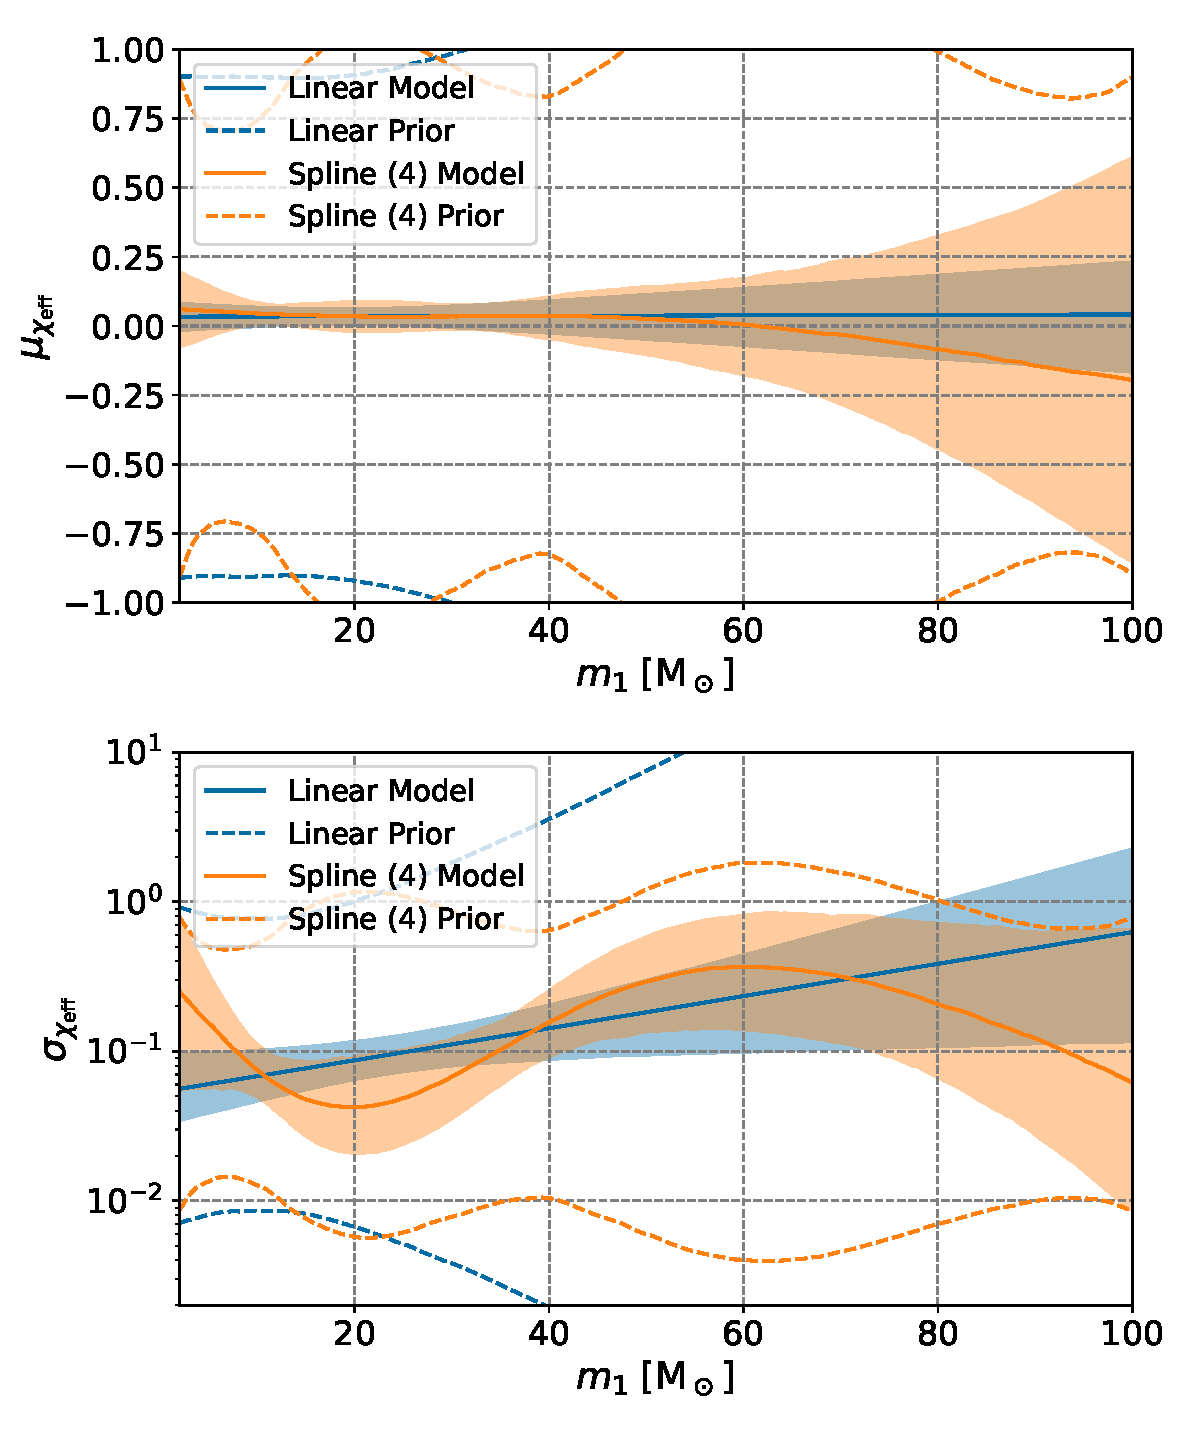
\includegraphics[width=0.9\linewidth]{chieff_m_GWTC3_linear_v_4nodes_unccut.pdf}
    \caption{A comparison between the linear model and 4 node spline model for correlation between $\chieff$ and primary mass, inferred using \ac{GWTC-3}. Solid lines represent the median, while the shaded region represents the central 90\% credible interval, and the dashed lines show the boundary of the prior 90\% interval. The upper panel shows the mean of the $\chieff$ Gaussian as a function of primary mass $m_1$, while the lower panel represents the standard deviation of the $\chieff$ distribution.}
    \label{fig:chieff_m_s4_v_linear}
\end{figure}

Using the same spline approach described above, we place nodes between $m_{\rm 1, min} = 2$ and $m_{\rm 1, max} = 100$, linearly spaced in $m_1^{1/3}$. A uniform node spacing doesn't easily allow for structure at $\sim 10-30 \Msun$, which we would like to probe.
% too much emphasis on the high mass region where a flexible model for the spin population is poorly constrained. 
Instead, linearly spaced in $m_1^{1/3}$ clusters nodes towards $m_1 \sim 10-30 \Msun$, which we found to be satisfactory. 
\begin{align}
\mu(\theta) &= S\left(m_1\;|\;(2,\mu_{\chieff:0}), ..., (100,\mu_{\chieff:N})\right) \nn \\
\ln \sigma(\theta) &= S\left(m_1\;|\; (2,\ln \sigma_{\chieff:0}), ..., (100,\ln \sigma_{\chieff:N})\right).
\label{eq:chieff_m_spline}
\end{align}
We show a comparison between the spline model with 4 nodes and the linear model, in Fig. \ref{fig:chieff_m_s4_v_linear}. The linear model and spline models appear broadly consistent; indeed the model evidences do not show any preference for one model over another (see the appendix, Fig. \ref{fig:chieff_evidences}. We also show the results for all spline runs in Fig. \ref{fig:chieff_correlations} in the appendix). 
\begin{figure}[h!]
    \centering
    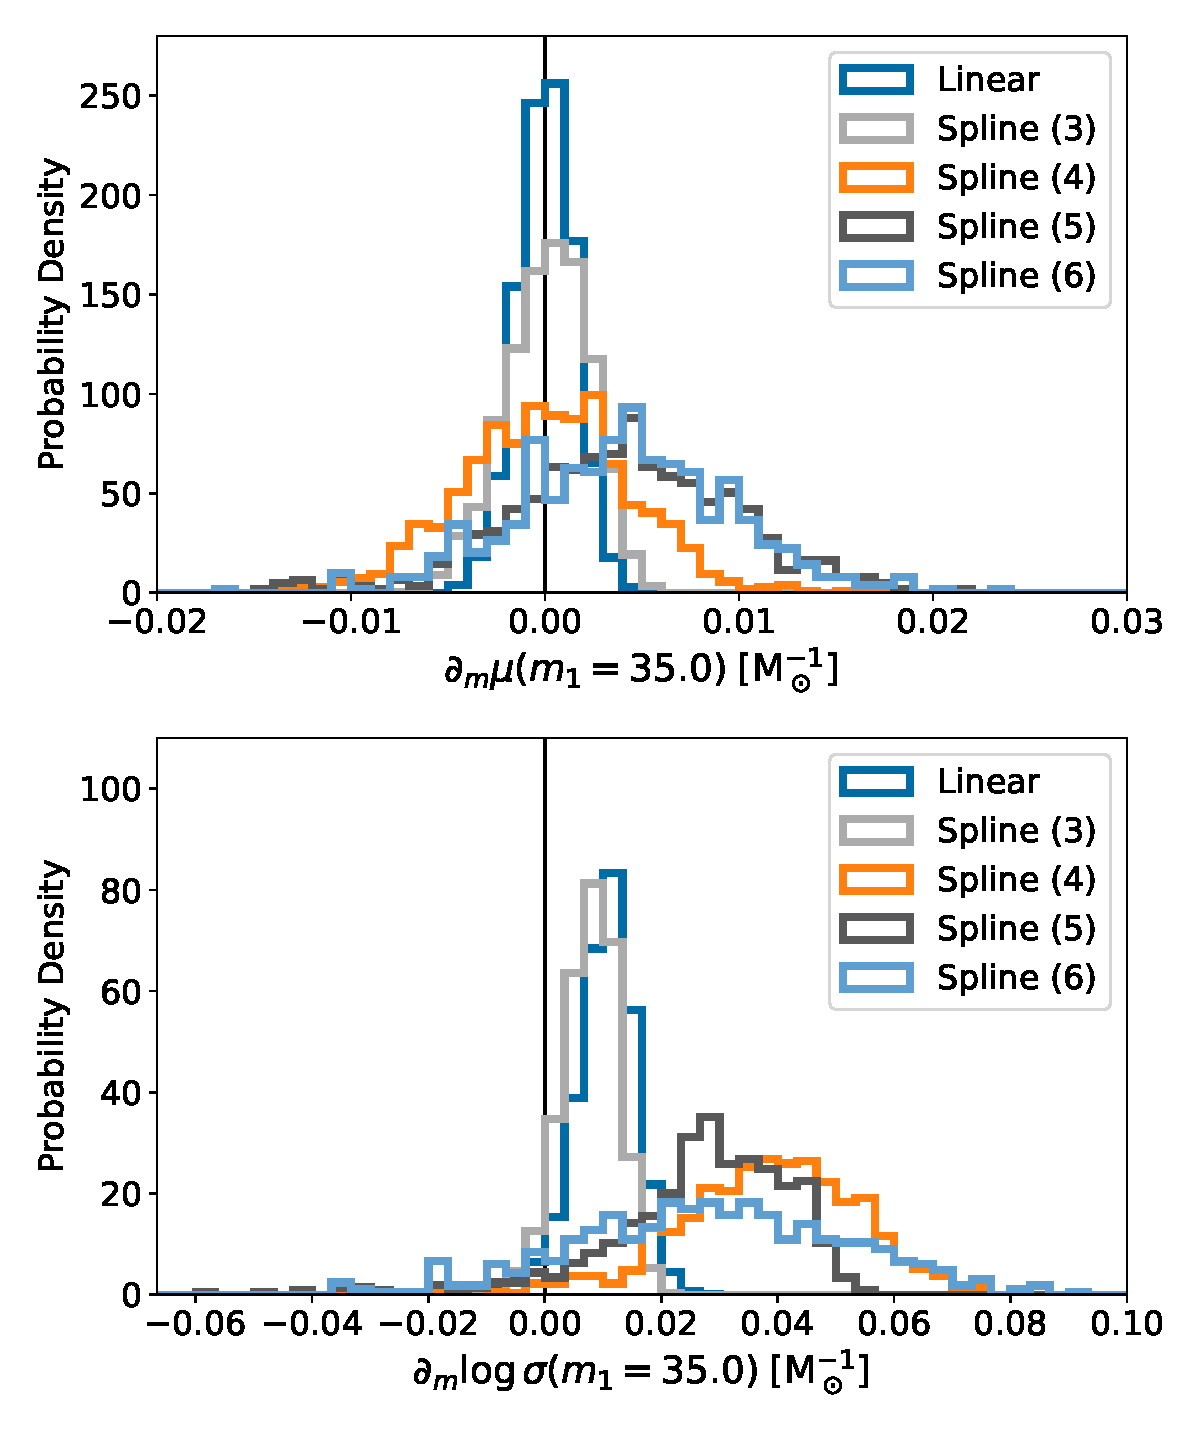
\includegraphics[width=0.9\linewidth]{chieff_m_GWTC3_m35.0_slopes_unccut_1.pdf}
    \caption{Posteriors on the derivative of the mean and width of the Gaussian as a function of primary mass. Each posterior is broadly consistent, with varying levels of confidence that the slope is greater than zero. The derivative of the mean at $m_0=35\Msun$ has nearly equal support for being positive of negative, while the derivative of the width is positive at $\sim 85-99.7\%$ confidence for each model.}
    \label{fig:chieff_m_slope}
\end{figure}

We also compute the slope of the mean and width at the fiducial value $m_1^* = 35 \Msun$, and here we find stronger evidence for a positive slope in some spline models than in the linear model. We chose $m_1^* = 35 \Msun$ to coincide roughly with the location of the Gaussian ``peak'' in the primary mass distribution~\cite{Talbot:2018cva, KAGRA:2021duu}, and so represents a physically interesting region of parameter space. The linear model finds a broadening at higher primary masses with significance $\sim 93\%$, while the spline models vary in significance, the model with 4 nodes notably exhibits a broadening at $98.7\%$ credence. We show posteriors on the slope at $m_1^* = 35\Msun$ in Fig. \ref{fig:chieff_m_slope}. 

\subsection{Inferences on \ac{GWTC-3}, extra analyses and evidences}
\label{app:extra_analysis}
We also run each correlation inference with 3-6 nodes for the mean and standard deviation spline functions. For the $\chieff-q$ correlation, we show the constraints on the mean and standard deviation functions in Fig. \ref{fig:chieff_evidences}.
We do not observe any strong preference for a including more nodes in the spline correlation functions; there is a generic ``Occam's penalty'' for including more nodes beyond what is necessary to appropriately fit the data. We show the evidence of the \ac{GWTC-3} data given all our correlation models in Fig. \ref{fig:chieff_evidences}; note the evidences are still inconclusive at this stage, though a correlation with mass ratio is somewhat preferred. 

\begin{figure}
    \centering
    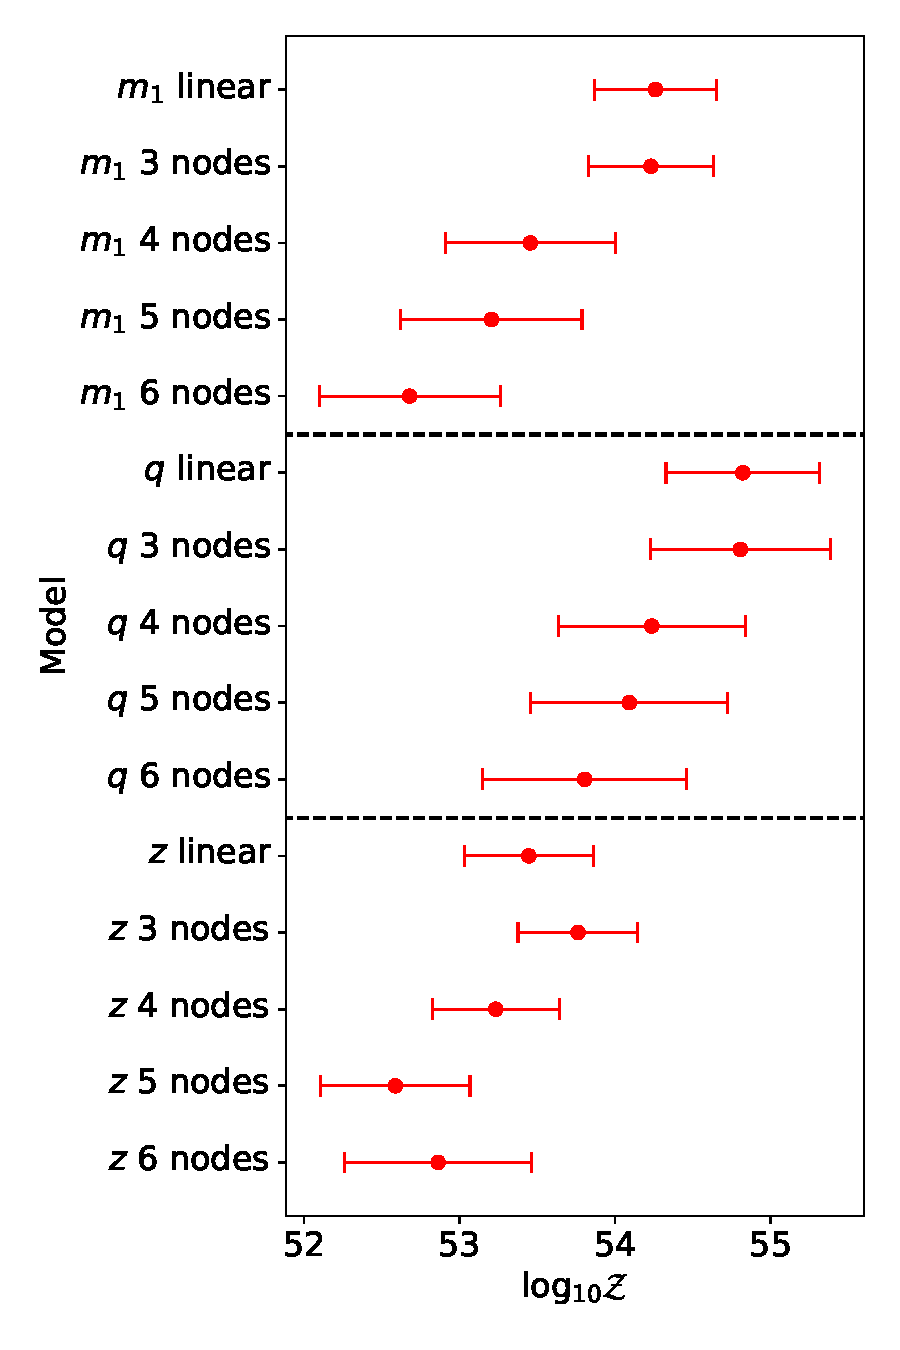
\includegraphics[width=0.9\linewidth]{GWTC3_spline_evidences.pdf}
    \caption{Evidences of the \ac{GWTC-3} catalog given each of the $\chieff$ correlation models. Evidence uncertainties include the average Monte Carlo uncertainty intrinsic to the likelihood estimator, added in quadrature with the nested sampling uncertainty of {\tt Dynesty}.}
    \label{fig:chieff_evidences}
\end{figure}

\begin{figure*}
    \centering
    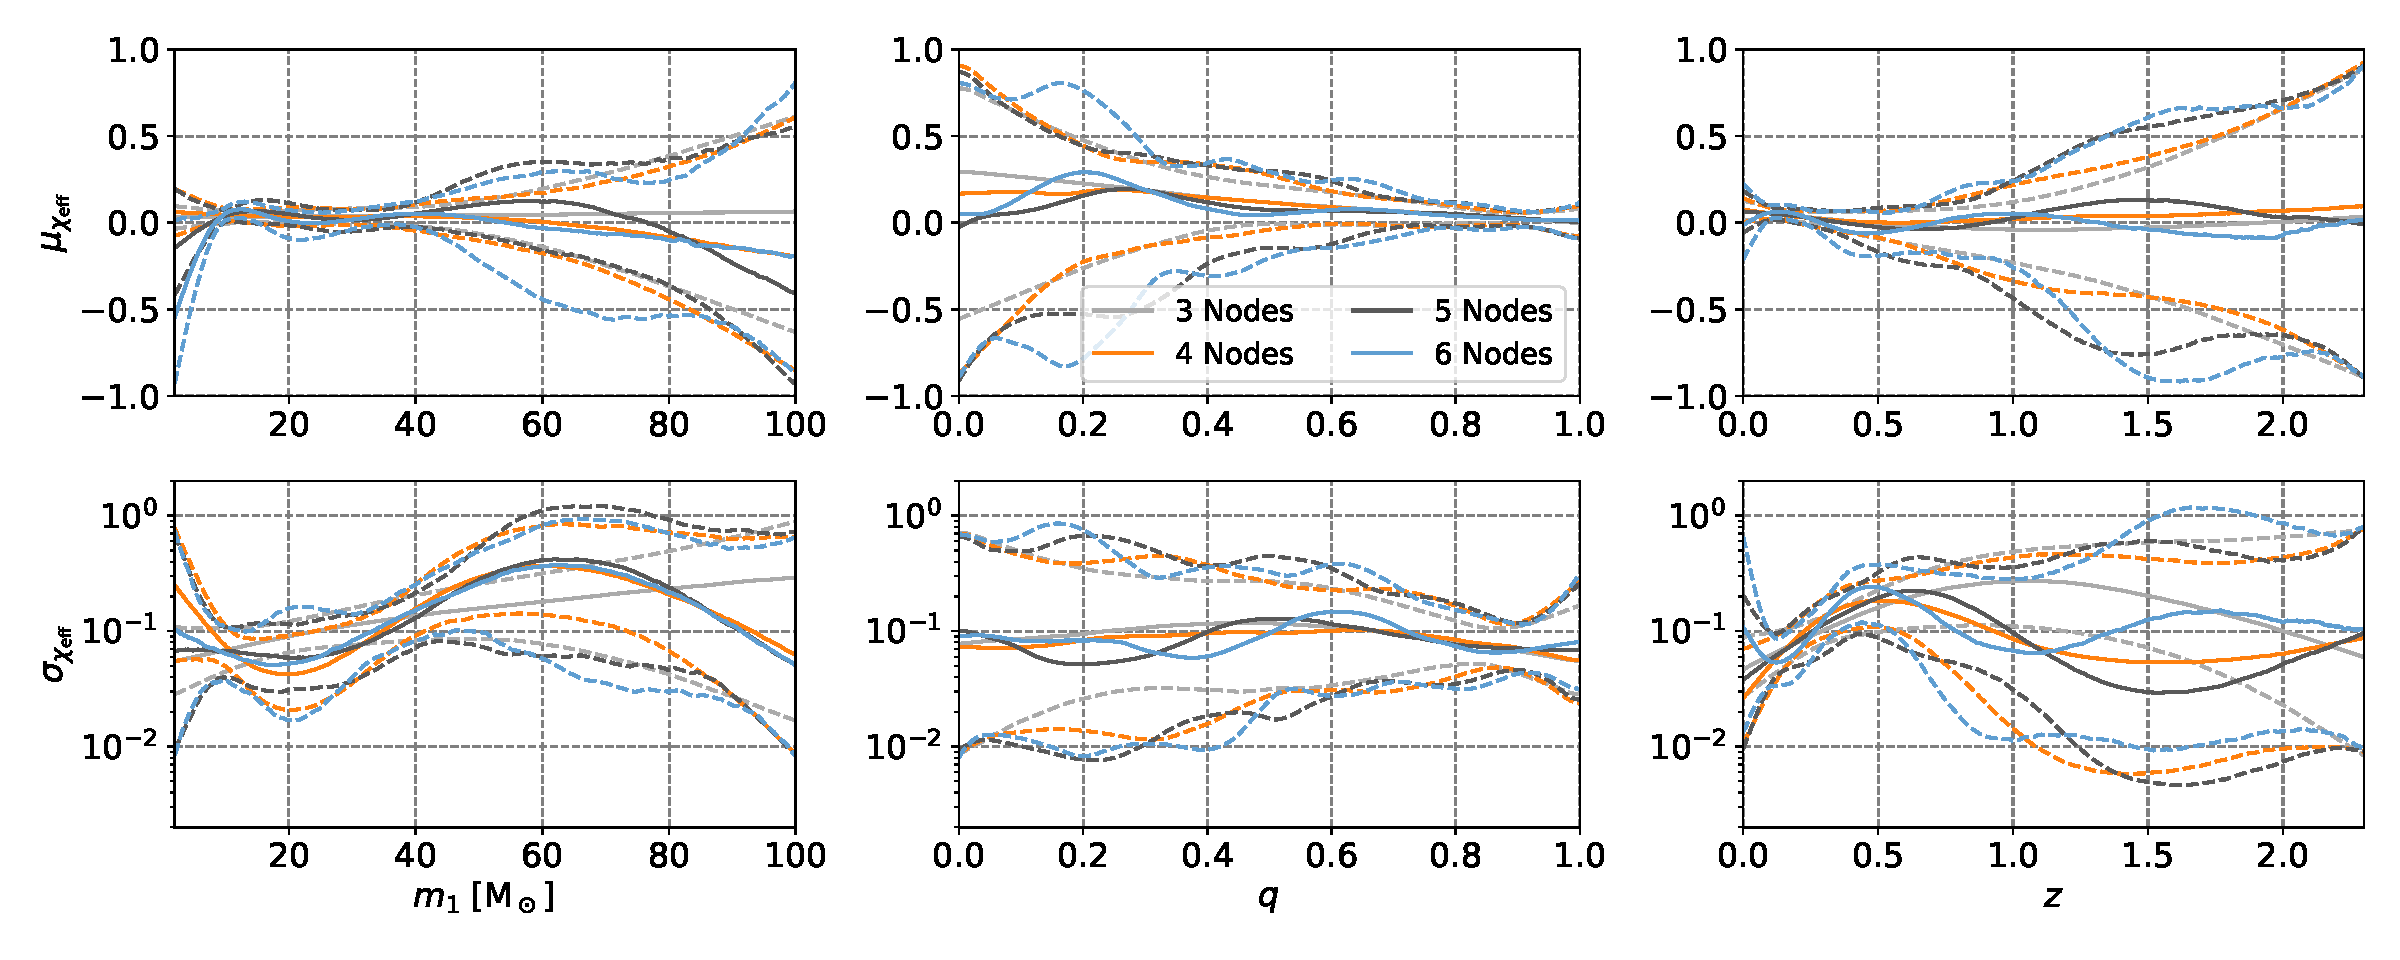
\includegraphics[width=0.95\linewidth]{GWTC3_all_spline_correlations_unccut_1.pdf}
    \caption{Spline correlations between $\chieff$ and each parameter we studied, primary mass $m_1$ (left column), mass ratio $q$ (center), and redshift $z$ (right). Solid lines represent the median, while the dashed lines represent the boundaries of the central 90\% credible interval. The upper panels represents the mean of the $\chieff$ Gaussian as a function of each parameter, while the lower panels represents the standard deviation of the $\chieff$ distribution.}
    \label{fig:chieff_correlations}
\end{figure*}


\renewcommand{\arraystretch}{1.5}
\begin{table*}
    \centering
    \begin{tabular}{|c|c|c|c|}
       \hline & $m_1$ (at $m_1^* = 35\Msun$) & $q$ (at $q^* = 0.9$) & $z$ (at $z^* = 0.2$)\\
       \hline Linear & \begin{tabular}{@{}c@{}} $p(\partial_m \mu > 0) = 53.9\%$ \\ $p(\partial_m \sigma > 0) = 93.2\%$ \end{tabular} & \begin{tabular}{@{}c@{}} $p(\partial_q \mu > 0) = 2.5\%$ \\ $p(\partial_q \sigma > 0) = 41.7\%$ \end{tabular} & \begin{tabular}{@{}c@{}} $p(\partial_z \mu > 0) = 16.2\%$ \\ $p(\partial_z \sigma > 0) = 92.7\%$ \end{tabular} \\
       \hline Spline (3) & \begin{tabular}{@{}c@{}} $p(\partial_m \mu > 0) = 55.0\%$ \\ $p(\partial_m \sigma > 0) = 89.5\%$ \end{tabular} & \begin{tabular}{@{}c@{}} $p(\partial_q \mu > 0) = 13.4\%$ \\ $p(\partial_q \sigma > 0) = 33.0\%$ \end{tabular} & \begin{tabular}{@{}c@{}} $p(\partial_z \mu > 0) = 14.2\%$ \\ $p(\partial_z \sigma > 0) = 95.6\%$ \end{tabular} \\
       \hline Spline (4) & \begin{tabular}{@{}c@{}} $p(\partial_m \mu > 0) = 60.5\%$ \\ $p(\partial_m \sigma > 0) = 98.7\%$ \end{tabular} & \begin{tabular}{@{}c@{}} $p(\partial_q \mu > 0) = 18.7\%$ \\ $p(\partial_q \sigma > 0) = 44.5\%$ \end{tabular} & \begin{tabular}{@{}c@{}} $p(\partial_z \mu > 0) = 19.6\%$ \\ $p(\partial_z \sigma > 0) = 98.0\%$ \end{tabular} \\
       \hline Spline (5) & \begin{tabular}{@{}c@{}} $p(\partial_m \mu > 0) = 78.3\%$ \\ $p(\partial_m \sigma > 0) = 95.7\%$ \end{tabular} & \begin{tabular}{@{}c@{}} $p(\partial_q \mu > 0) = 21.7\%$ \\ $p(\partial_q \sigma > 0) = 58.1\%$ \end{tabular} & \begin{tabular}{@{}c@{}} $p(\partial_z \mu > 0) = 17.0\%$ \\ $p(\partial_z \sigma > 0) = 88.8\%$ \end{tabular} \\
       \hline Spline (6) & \begin{tabular}{@{}c@{}} $p(\partial_m \mu > 0) = 77.8\%$ \\ $p(\partial_m \sigma > 0) = 93.6\%$ \end{tabular} & \begin{tabular}{@{}c@{}} $p(\partial_q \mu > 0) = 30.0\%$ \\ $p(\partial_q \sigma > 0) = 65.5\%$ \end{tabular} & \begin{tabular}{@{}c@{}} $p(\partial_z \mu > 0) = 5.9\%$ \\ $p(\partial_z \sigma > 0) = 98.6\%$ \end{tabular} \\
       \hline 
    \end{tabular}
    \caption{Credibility of a positive slope in the evolution of the mean (denoted $\delta \mu > 0$) at the fiducial value, and of a positive slope in the evolution of the width (denoted $\delta \sigma > 0$). The column on the left is the model assumed, where ``Spline ($N$)'' refers to the spline model using $N$ nodes. In each cell, the top line represents the credibility of a positive slope in the mean, and the bottom line represents the same quantity for the width.}
    \label{tab:slope_significance}
\end{table*}

\subsection{Nonlinear Correlation in $\chieff-z$}
\label{app:nonlinear_z}
\begin{figure}
    \centering
    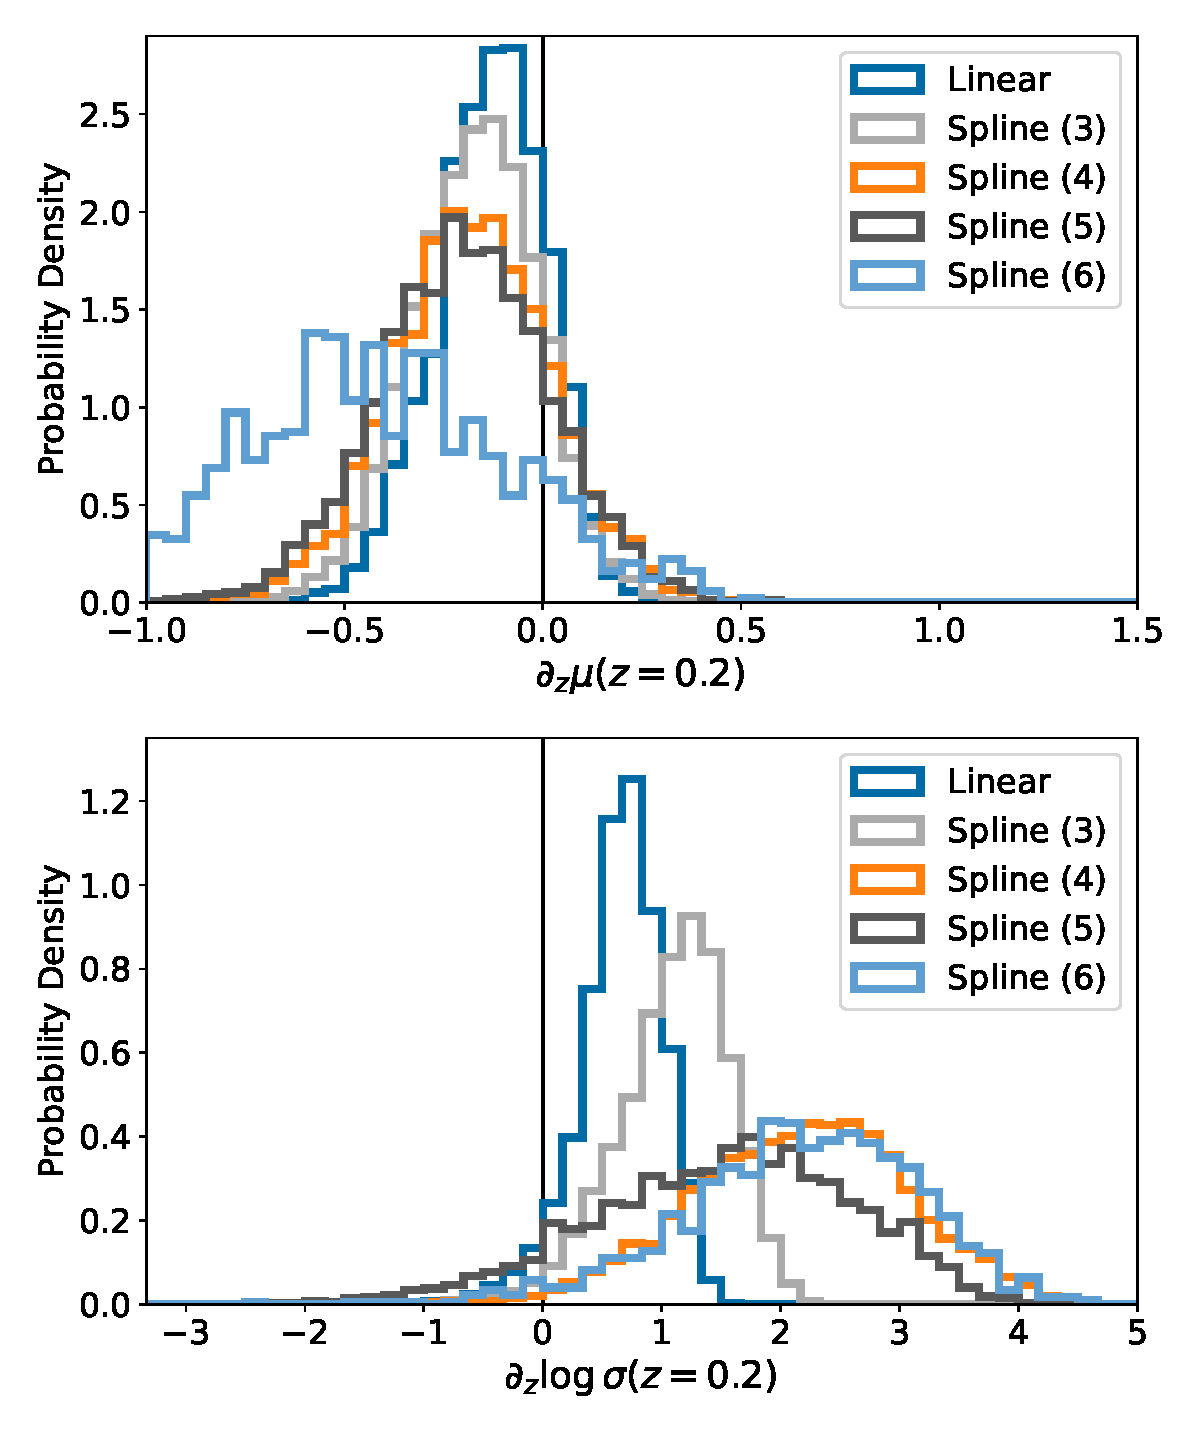
\includegraphics[width=0.9\linewidth]{chieff_z_GWTC3_z0p2_slopes_unccut_1.pdf}
    \caption{Posteriors on the derivative of the mean and width of the Gaussian with respect to redshift at $z^* = 0.2$, inferred on \ac{GWTC-3} data. Each posterior is consistent, with varying levels of confidence that the slope is greater than zero.}
    \label{fig:chieff_z_slope}
\end{figure}


To study the potential risk of inferring a nonlinear correlation a \ac{GWTC-3}-like catalog from a linearly correlated Universe, we used 12 sets of 69 detections drawn from a uncorrelated Universe observed with Hanford and Livingston in O4-like PSDs \cite{O3_psds}, in a similar process to the method presented in \S \ref{sec: spline o4_projections}. These synthetic events were injected from a linearly correlated Universe (namely, uncorrelated with slope zero), with a mean $\mu_{\chieff} = 0.06$ and width $\sigma_{\chieff} = 0.11$, and the same thresholds, waveforms, and PE techniques described in \S \ref{sec: spline o4_projections}. Then, we infer the $\chieff$ correlation with respect to the redshift $z$ for each synthetic catalog, using the method we introduced in \S \ref{sec: spline GWTC3_results}. We compute the instantaneous slope at the first three nodes for each hyperposterior sample, and can then estimate the \ac{JS} divergence between the posteriors of the slopes at neighboring nodes. 

We also show the slope posteriors at a fiducial value $z^*=0.2$ in Fig. \ref{fig:chieff_z_slope}. We avoid choosing $z^*=0$, as the data is uninformative in the limit of $z\to 0$ for the same reason it is uninformative for $q\to 0$. While some of the 69 BBH events are closer than others, none of them are consistent with being at $z\to 0$, and indeed it is baked into the population model where the probability density at a given redshift is proportional to the differential comoving volume $p(z) \propto \frac{dV_c}{dz}$ to have zero support at $z\to 0$ \cite{Hogg:1999ad, Fishbach:2018edt}. In other words, a flexible $z-\chieff$ correlation model, in particular spline models with appropriate node density and placement, will increase in uncertainty as $z\to 0$. Indeed, we observe this to some degree in each spline model in Fig. \ref{fig:chieff_correlations}, but it is especially clear in the spline model with 5 nodes. 

We also should note the significance of broadening with redshift using the linear model is only 92.7\%, while Ref.~\cite{Biscoveanu:2022qac} inferred a broadening at 98.6\% credibility. We checked various differences between our analyses, and discovered that this difference arises from how selection effects are estimated. In particular, Ref.~\cite{Biscoveanu:2022qac} assumes a semi-analytic threshold on the network SNR $\rho_{\rm net} > 9$ for O1 and O2 events, while we use a threshold of $\rho_{\rm net} > 10$, following Ref.~\cite{KAGRA:2021duu}.

\subsection{Node Placement and Bias in Mock Catalogs}
\label{app:node_placement_bias}
In \S \ref{sec: spline o4_projections} we study a Universe with a nonlinear correlation in the $\chieff-q$ plane. We find that, when we fix the x-axis positions of the nodes to be different than the true node positions, we may recover some bias in the inference.

Specifically, the results in Fig. \ref{fig:chieff_q_mock_catalog_s4_v_linear} highlight one of the drawbacks for using spline models. Fitting a spline model to a smooth function often results in extraneous structure, bumps that the spline function cannot remove entirely due to its functional form \cite{Farah:2023vsc}. In the case of the mock catalog we simulated, the correlation is created using a spline node placement (Table \ref{tab:true_hyper}) different from the spline node placement scheme we recover with. Because of this, the spline cannot simultaneously fit the correlation in the region of near equal mass ratio while also effectively fitting the region of more extreme mass ratios, and so it must compromise with a suboptimal fit across the parameter space. Hence the spline model ``wiggles'' when it ideally should be smooth.  %, see the appendix. Fig. \ref{fig:true_vs_false_node_q}.

Because we are not yet in the limit of infinitely many nodes (we use 4 nodes in this inference), the spline functions are not perfectly flexible. More nodes are inherently more flexible, and so would presumably do a better job at fitting the correlation. Similarly, using a correct node placement scheme should also improve the fit. Indeed, we find that when we analyze the mock catalog using the same node positions as the true correlation (Table \ref{tab:true_hyper}), the inferred correlation is closer to the truth. This highlights the importance of either running with multiple node counts and placement schemes, or marginalizing over the node x-axis positions as well.


% \begin{figure}
%     \centering
%     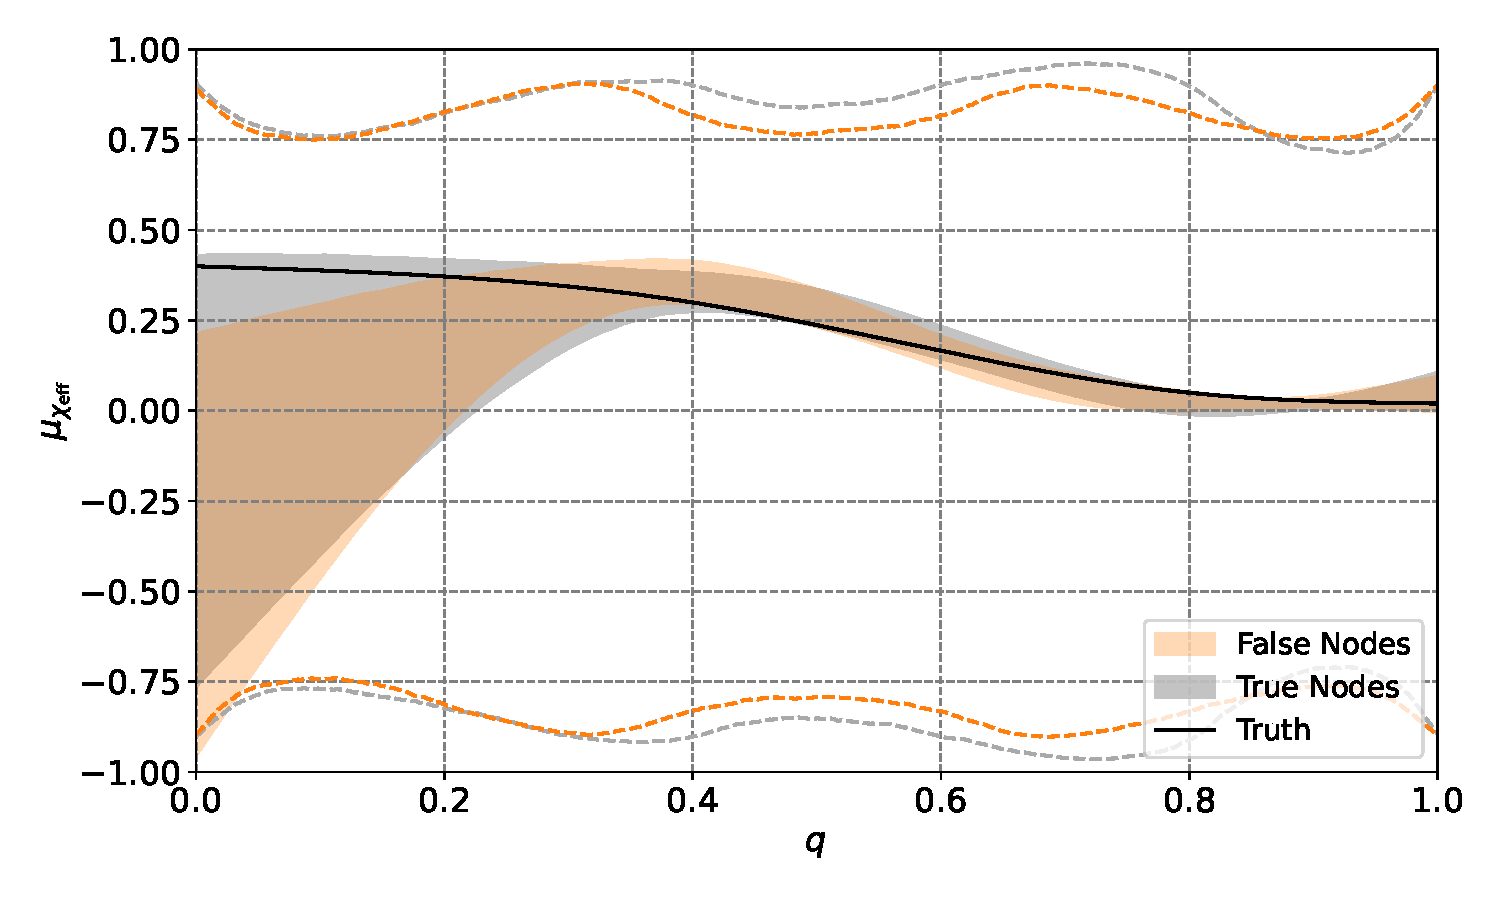
\includegraphics[width=0.9\linewidth]{mock_catalogs_chieff_q_GWTC3_q_tvf_nodes_mean.pdf}
%     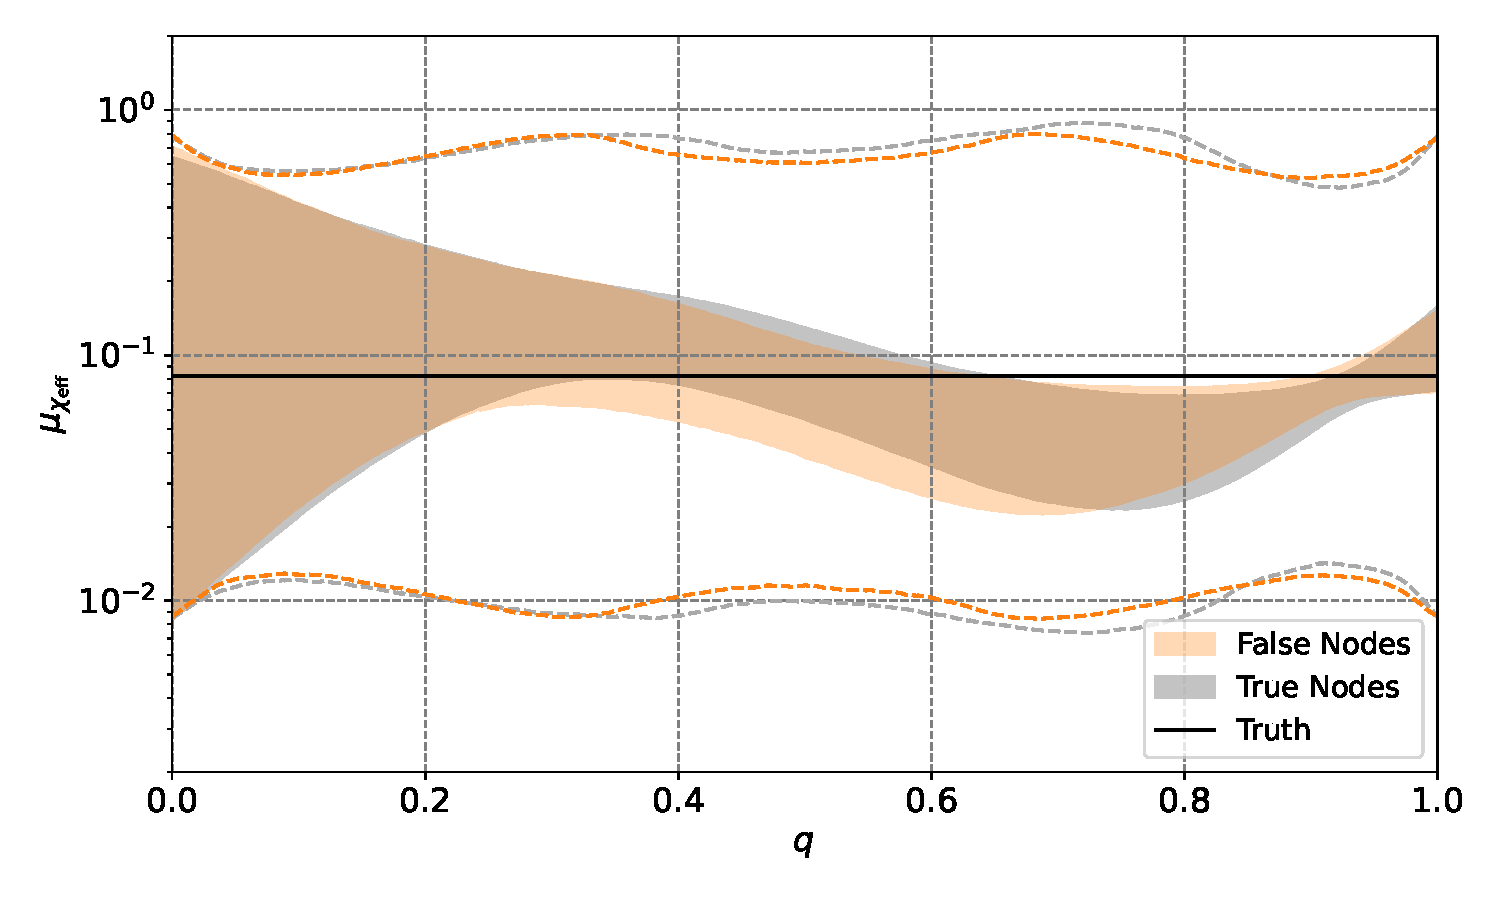
\includegraphics[width=0.9\linewidth]{mock_catalogs_chieff_q_GWTC3_q_tvf_nodes_sig.pdf}
%     \caption{Inferred mean and width of the $\chieff$ distribution as a function of mass ratio $q$ on the mock catalog with 400 detections. In orange are the 90\% credible interval when using the false node placement scheme, uniform in mass ratio. In dark grey is the credible interval using the true node placements; note the true node placement results in an improved fit to the true correlation.}
%     \label{fig:true_vs_false_node_q}
% \end{figure}


\printbibliography[heading=subbibliography]
\end{refsection}

%\end{document}  % commented out — document ends in MIT-Thesis.tex